\documentclass[aspectratio=169,10pt]{beamer}

% ==============================================================================
% THEME & STYLING (Cardiovascular Clinical-AI Palette)
% ==============================================================================
\usepackage{xcolor}
\definecolor{NavyPrimary}{HTML}{1E3A8A}    % Deep Clinical Navy
\definecolor{CyanAccent}{HTML}{0284C7}     % Signal Cyan
\definecolor{SlateDark}{HTML}{0F172A}      % Text Dark Slate
\definecolor{SlateMuted}{HTML}{64748B}     % Muted Slate
\definecolor{LightBg}{HTML}{F8FAFC}        % Subtle Card Background
\definecolor{BorderColor}{HTML}{E2E8F0}    % Clean Border
\definecolor{AlertRed}{HTML}{B91C1C}       % Alert Red
\definecolor{SuccessGreen}{HTML}{15803D}   % Success Green

\usetheme{default}
\usecolortheme{default}

% Typography & Colors
\setbeamercolor{normal text}{fg=SlateDark,bg=white}
\setbeamercolor{frametitle}{fg=NavyPrimary,bg=white}
\setbeamercolor{title}{fg=NavyPrimary}
\setbeamercolor{subtitle}{fg=SlateMuted}
\setbeamercolor{structure}{fg=NavyPrimary}
\setbeamercolor{block title}{fg=white,bg=NavyPrimary}
\setbeamercolor{block body}{fg=SlateDark,bg=LightBg}
\setbeamercolor{block title alerted}{fg=white,bg=AlertRed}
\setbeamercolor{block body alerted}{fg=SlateDark,bg=LightBg}
\setbeamercolor{block title example}{fg=white,bg=CyanAccent}
\setbeamercolor{block body example}{fg=SlateDark,bg=LightBg}

% Frame styling
\setbeamertemplate{navigation symbols}{}
\setbeamertemplate{frametitle}{
  \vspace{0.4em}
  {\large\textbf{\insertframetitle}}\\[-0.2em]
  {\scriptsize\color{SlateMuted}\insertframesubtitle}
  \vspace{0.2em}
  {\color{BorderColor}\hrule height 0.55pt}
  \vspace{0.2em}
}

% Footline
\setbeamertemplate{footline}{
  \leavevmode%
  \hbox{%
    \begin{beamercolorbox}[wd=0.75\paperwidth,ht=2.5ex,dp=1ex,left]{author in head/foot}%
      \hspace*{0.8cm}\scriptsize\color{SlateMuted}Sunnybrook Arrhythmia Trial Protocol $\cdot$ 12-Lead AI Integration
    \end{beamercolorbox}%
    \begin{beamercolorbox}[wd=0.25\paperwidth,ht=2.5ex,dp=1ex,right]{title in head/foot}%
      \scriptsize\color{SlateMuted}\insertframenumber{} / \inserttotalframenumber\hspace*{0.8cm}
    \end{beamercolorbox}%
  }%
  \vspace{0.2cm}
}

% Required Packages
\usepackage{graphicx}
\usepackage{booktabs}
\usepackage{amsmath,amssymb}
\usepackage{microtype}
\graphicspath{{figures/}}

% Metadata
\title{Integrating 12-Lead AI Reconstruction into the Sunnybrook Wearable AF Trial}
\author{\textbf{Mithun Manivannan, BSc} \and \textbf{Alex Mariakakis, PhD} \and \textbf{Christopher Cheung, MD, MPH}}
\institute{Sunnybrook Research Institute \quad | \quad Department of Computer Science, University of Toronto}
\date{Research Strategy Meeting \quad | \quad September 2026}

\begin{document}

% ------------------------------------------------------------------------------
% Slide 1: Title Slide
% ------------------------------------------------------------------------------
\begin{frame}[plain]
  \vspace{1.5em}
  \centering
  {\LARGE\textbf{\color{NavyPrimary}Integrating 12-Lead AI Reconstruction\\[0.15em]into the Sunnybrook Wearable AF Trial}}\\[0.6em]
  
  \begin{columns}[c]
    \begin{column}{0.85\textwidth}
      \centering
      \footnotesize
      Christopher Cheung, MD, MPH $\cdot$ Alex Mariakakis, PhD $\cdot$ Mithun Manivannan, BSc\\
      \textit{Division of Cardiology, Sunnybrook Health Sciences Centre $\cdot$ Department of Computer Science, University of Toronto}
    \end{column}
  \end{columns}
  \vspace{1.2em}
  {\color{BorderColor}\rule{0.7\textwidth}{0.55pt}}\par
  \vspace{0.6em}
  {\scriptsize\color{SlateMuted}Protocol: \textit{Evaluation of Wearable/FitBit Monitoring to Detect Recurrent Atrial Fibrillation} (v1.1)}\par
  \note{
    Good morning Chris, good morning Alex. The purpose of today's meeting is straightforward: we already have an established clinical trial protocol—the Sunnybrook FitBit/Wearable ECG Study, authored by Chris, Alex, and our team.
    Our goal today is to establish how we can cleanly integrate our single-lead to 12-lead AI reconstruction research into this existing trial as a pre-specified secondary translational aim, without adding patient burden or endangering the primary clinical trial endpoints.
  }
\end{frame}

% ------------------------------------------------------------------------------
% Slide 2: Purpose of Today's Meeting
% ------------------------------------------------------------------------------
\begin{frame}{Purpose of Today's Meeting}{Protocol alignment and study integration}
\begin{columns}[T]
  \begin{column}{0.32\textwidth}
    \begin{block}{\textbf{Clinical Trial Foundation}}
      \scriptsize
      \begin{itemize}
        \item Established protocol (Version 1.1, October 2025).
        \item Target cohort: persistent AF patients undergoing catheter ablation.
        \item Reference standard: 14-day continuous CardioSTAT patch at 3 and 6 months.
        \item Primary clinical endpoint: time to confirmed AF recurrence.
      \end{itemize}
    \end{block}
  \end{column}
  \begin{column}{0.32\textwidth}
    \begin{block}{\textbf{Reconstruction Constraints}}
      \scriptsize
      \begin{itemize}
        \item 12-lead reconstruction from single-lead input is underdetermined.
        \item Precordial leads exhibit amplitude and morphology errors under direct projection.
        \item Diagnostic reconstruction cannot serve as a primary clinical endpoint.
        \item Separates clinical trial validity from exploratory AI evaluation.
      \end{itemize}
    \end{block}
  \end{column}
  \begin{column}{0.32\textwidth}
    \begin{block}{\textbf{Translational Integration}}
      \scriptsize
      \begin{itemize}
        \item Routine outpatient visits already include scheduled 12-lead ECGs.
        \item Synchronous smartwatch and 12-lead acquisition adds $\le 5$ minutes.
        \item Evaluates reconstruction and biomarker recovery as a secondary aim.
        \item Generates a prospectively paired clinical and wearable dataset.
      \end{itemize}
    \end{block}
  \end{column}
\end{columns}
\vspace{0.4em}
\centering
\scriptsize
{\color{NavyPrimary}Objective: Align on the secondary data collection protocol and freeze translational evaluation metrics.}
\note{
  Here is the layout for today.
  Box 1 is our foundation: Chris's clinical protocol is locked. It evaluates smartwatch monitoring versus continuous CardioSTAT patch for post-ablation AF recurrence.
  Box 2 is our methodological reality check: we know 12-lead reconstruction does not work with uniform diagnostic precision across all leads and patients; staking the trial on reconstruction would be scientifically unsound.
  Box 3 is our opportunity: during routine clinical visits, we can capture simultaneous paired watch and 12-lead recordings. This establishes a publishable secondary translational AI aim while protecting the primary trial.
}
\end{frame}

% ------------------------------------------------------------------------------
% Slide 3: The Established Clinical Protocol (v1.1)
% ------------------------------------------------------------------------------
\begin{frame}{The Established Clinical Protocol (v1.1)}{Protocol v1.1 design and endpoints}
\begin{columns}[T]
  \begin{column}{0.48\textwidth}
    \begin{block}{\textbf{Trial Design \& Patient Population}}
      \scriptsize
      \begin{itemize}
        \setlength{\itemsep}{0.2em}
        \item Single-center prospective cohort at Sunnybrook Arrhythmia Clinic.
        \item Patients aged $\ge 18$ with persistent AF undergoing catheter ablation or cardioversion.
        \item Smartwatch monitoring: daily 30-second ECG and automated rhythm notifications for 6 months.
        \item Reference standard: 14-day continuous CardioSTAT patch at 3 and 6 months post-procedure.
      \end{itemize}
    \end{block}
  \end{column}
  \begin{column}{0.48\textwidth}
    \begin{block}{\textbf{Endpoints \& Sample Size}}
      \scriptsize
      \begin{itemize}
        \setlength{\itemsep}{0.2em}
        \item Primary outcome: time to recurrent AF detection (smartwatch vs. patch).
        \item Secondary clinical outcomes: heart rate trends, heart rate variability, and cumulative AF burden.
        \item Sample size: $N = 96$ patients (80\% power, $\alpha=0.05$, 10\% non-inferiority margin).
        \item Vanguard phase: initial 20 consecutive patients to assess protocol adherence and data pipeline.
      \end{itemize}
    \end{block}
  \end{column}
\end{columns}
\vspace{0.4em}
\centering
\scriptsize
{\color{NavyPrimary}Primary trial endpoints and clinical workflows remain unchanged under this proposal.}
\note{
  Let us ground ourselves in the exact text of Protocol Version 1.1.
  Chris designed this study to evaluate whether daily smartwatch ECG recordings and photoplethysmography irregular rhythm notifications detect recurrent AF earlier than standard-of-care intermittent patch monitoring.
  Patients receive a 14-day CardioSTAT patch at 3 months and 6 months post-procedure, with clinical-grade de-identified reports from iCentia.
  The primary endpoint is time to AF recurrence. The sample size is 96 patients, starting with a 20-patient vanguard.
  This clinical core remains completely untouched.
}
\end{frame}

% ------------------------------------------------------------------------------
% Slide 4: Related & Prior Work
% ------------------------------------------------------------------------------
\begin{frame}{Related \& Prior Work}{Limitations of existing protocols motivating prospective paired acquisition}
\vspace{-0.3em}
\centering
{\renewcommand{\arraystretch}{0.78}
\resizebox{0.97\textwidth}{!}{%
\tiny
\begin{tabular}{@{}p{3.0cm}p{4.2cm}p{4.2cm}p{4.6cm}@{}}
\toprule
\textbf{Study} & \textbf{Approach} & \textbf{Key Finding} & \textbf{Limitation} \\
\midrule
\textbf{Wearable AF Detection} & & & \\[0.1em]
\quad Abu-Alrub et al. (2022) & Smartwatch single-lead AF detection; 6-month post-ablation & Sensitivity $\approx 94\%$ for AF vs.\ CardioSTAT patch & No 12-lead integration; cannot assess repolarization or conduction \\[0.2em]
\quad Cheung et al. (2025) & Fitbit vs.\ CardioSTAT patch in post-ablation cohort & Comparable AF recurrence yield at 3 and 6 months & No ECG morphology analysis; single-lead rhythm only \\
\midrule
\textbf{Single-Lead Reconstruction} & & & \\[0.1em]
\quad Ansari, Rogers et al.\ (\textit{Circulation} 2026) & Auxiliary 12-lead head on ICM/CareLink lead; 3DRECON-QT & Spatial conditioning $\uparrow$ biomarker correlation ($r$: $0.04\!\to\!0.73$) & Retrospective archive ($N=26$); $\pm 7$-day offset; subcutaneous ICM, not surface wearable \\[0.2em]
\quad Presacan et al.\ (\textit{Comm.\ Medicine} 2025) & DL 12-lead recovery from single precordial & $r > 0.80$ on limb leads & Amplitude compression on V2--V4; evaluated on synthetic-masked PTB-XL only \\[0.2em]
\quad Strodthoff et al.\ (2021) & PTB-XL benchmark with masked-lead evaluation & Transformer models $r \approx 0.85$ on standard leads & Closed-loop: train/test on same masking distribution; does not reflect real deployment \\
\midrule
\textbf{Wearable Domain Gap} & & & \\[0.1em]
\quad Hu et al.\ (2026) & Hospital Lead I vs.\ wrist Lead I in 120 patients & Disagreement $>0.3$\,mV along precordial-sensitive axes & Observational only; no paired dataset released; no reconstruction model tested \\[0.2em]
\quad General literature & All models trained on hospital 12-lead corpora & Wet gel, supine, artifact-free training data & No published model validated on real smartwatch (dry, wrist-mounted, DSP-filtered) signals \\
\bottomrule
\end{tabular}%
}}
\vspace{0.15em}
\begin{alertblock}{}
  \scriptsize
  No existing study evaluates reconstruction on a real wearable signal paired with a simultaneous clinical 12-lead ECG. This is the gap our Sunnybrook protocol addresses.
\end{alertblock}
\note{
  This slide covers the three main threads of prior work we build on, and their limitations.
  Thread 1: Wearable AF detection. Post-ablation smartwatch studies demonstrate high sensitivity for detecting AF recurrence. However, none integrate 12-lead ECG morphology analysis. The AF detection endpoint is well-established; the open question is whether wearable signals can carry additional diagnostic information beyond rhythm detection.
  Thread 2: Single-lead 12-lead reconstruction. The key paper is Ansari and Rogers in Circulation 2026. They trained an auxiliary 12-lead reconstruction head on signals from Medtronic CareLink ICMs. Their central finding—that spatial supervision strongly improves downstream biomarker correlation—is compelling. However, their retrospective paired cohort was only 26 patients with a temporal offset of up to 7 days between the ICM signal and the clinical 12-lead. That offset means physiological state could differ substantially. And critically, the ICM lead is a subcutaneous implanted device, not a surface wearable. Presacan 2025 showed amplitude compression and regression to the mean on precordial leads; Strodthoff 2021's benchmarks test on the same data distribution used for training.
  Thread 3: The wearable domain gap. Hu et al. in 2026 demonstrated empirically that hospital Lead I and wrist Lead I systematically disagree. The fundamental reason is physics: dry stainless-steel electrodes on the wrist have different contact impedance, different baseline wander, motion artifacts, and are processed through proprietary DSP. Every reconstruction model in the literature is trained exclusively on hospital 12-lead corpora. None have been validated on real smartwatch signals.
  Our Sunnybrook protocol is the first to collect a prospective, synchronous, real-wearable-to-12-lead paired dataset in a post-ablation AF cohort. That is both a methodological and a dataset contribution.
}
\end{frame}

% ------------------------------------------------------------------------------
% Slide 5: The Clean Integration: A Rigorous Two-Track Protocol
% ------------------------------------------------------------------------------
\begin{frame}{The Clean Integration: A Rigorous Two-Track Protocol}{Separation of primary clinical and secondary AI aims}
\begin{columns}[T]
  \begin{column}{0.48\textwidth}
    \begin{block}{\textbf{Track 1: Primary Clinical Aim}}
      \scriptsize
      \begin{itemize}
        \setlength{\itemsep}{0.2em}
        \item Does daily smartwatch monitoring improve time to detection of recurrent AF versus 14-day CardioSTAT patch?
        \item Reference standard: iCentia-analyzed CardioSTAT patch at 3 and 6 months.
        \item $N=96$ patients; 80\% power; 20-patient feasibility vanguard.
        \item Primary regulatory endpoint. Trial conclusions do not depend on AI performance.
      \end{itemize}
    \end{block}
  \end{column}
  \begin{column}{0.48\textwidth}
    \begin{block}{\textbf{Track 2: Secondary Translational AI Aim}}
      \scriptsize
      \textit{Core question: can we reconstruct a 12-lead ECG from a smartwatch in an AF population?}
      \vspace{0.3em}
      \begin{itemize}
        \setlength{\itemsep}{0.2em}
        \item Aim 2: Benchmark wearable-to-12-lead reconstruction in post-ablation patients --- including recordings captured during AF, immediately post-cardioversion, and in sinus rhythm.
        \item Aim 3: Track within-patient repolarization changes ($\Delta$QTc, P-wave remodeling) over 6 months using an in-clinic 12-lead prior.
        \item Exploratory endpoints; no impact on primary trial conclusions.
      \end{itemize}
    \end{block}
  \end{column}
\end{columns}
\vspace{0.3em}
\centering
\scriptsize
{\color{NavyPrimary}Track 1 guarantees clinical output regardless of AI results. Track 2 generates a dataset and benchmark that does not yet exist anywhere.}
\note{
  This architecture cleanly separates the two efforts.
  Track 1 is the primary clinical trial: time to recurrent AF detection, backed by the 14-day CardioSTAT patch. This guarantees the study will produce high-impact clinical papers regardless of AI performance.
  Track 2 is the secondary translational AI aim. The core question is whether we can reconstruct a 12-lead ECG from a wrist wearable signal specifically in an AF population. This is different from generic ECG reconstruction benchmarks, which are dominated by sinus rhythm recordings. Post-ablation patients will be recorded in multiple rhythm states: some in AF at baseline, some immediately post-cardioversion, and most at 3 and 6 months in sinus rhythm with varying degrees of atrial remodeling. That longitudinal rhythm variation is scientifically valuable and is not captured in any existing dataset.
}
\end{frame}

% ------------------------------------------------------------------------------
% Slide 6: The 3DRECON Methodology: Multitask Spatial Regularization
% ------------------------------------------------------------------------------
\begin{frame}{Multitask Auxiliary Supervision (Ansari et al., 2026)}{Spatial representation learning for single-lead models}
\begin{columns}[T]
  \begin{column}{0.48\textwidth}
    \begin{block}{\textbf{Stanford 3DRECON-QT Framework}}
      \scriptsize
      \begin{itemize}
        \setlength{\itemsep}{0.2em}
        \item Reference: Ansari, Rogers et al., \textit{Circulation} (January 2026).
        \item Multitask objective: simultaneously reconstruct 12 leads from synthetic ICM/cardiostat lead (voltage difference ) and estimate clinical biomarkers.
        \item Auxiliary 12-lead loss enforces 3D cardiac vector representations in the encoder.
        \item Removing spatial supervision reduced downstream biomarker correlation from $r = 0.73$ to $0.04$.
      \end{itemize}
    \end{block}
  \end{column}
  \begin{column}{0.48\textwidth}
    \begin{block}{\textbf{Application to Single-Lead AF Surveillance}}
      \scriptsize
      \begin{itemize}
        \setlength{\itemsep}{0.2em}
        \item Daily single-lead smartwatch ECG monitors for AF recurrence.
        \item Lead I captures frontal plane potentials, with limited sensitivity to orthogonal atrial vectors.
        \item Auxiliary 12-lead reconstruction head encourages representation of full 3D vector loops.
        \item Supports atrial feature extraction without altering primary single-lead inference inputs.
      \end{itemize}
    \end{block}
  \end{column}
\end{columns}
\vspace{0.4em}
\centering
\scriptsize
{\color{NavyPrimary}Auxiliary 12-lead reconstruction acts as an inductive regularizer during pretraining.}
\note{
  This slide connects our project to recent literature published in Circulation by Albert Rogers' group at Stanford (Ansari et al., 2026).
  Ansari developed 3DRECON-QT, showing that training an auxiliary 12-lead reconstruction head forces the single-lead encoder to learn 3D cardiac vector loops. In their ablation study, removing the 12-lead spatial conditioning collapsed downstream clinical biomarker prediction from r=0.73 down to 0.04.
  We apply this paradigm to our trial:
  At home, patients record daily single-lead smartwatch ECGs for our primary endpoint: time to AF recurrence.
  Lead I alone often misses vector components oriented perpendicular to the frontal plane.
  Training an auxiliary 12-lead reconstruction head helps the encoder preserve 3D atrial vector dynamics.
}
\end{frame}

% ------------------------------------------------------------------------------
% Slide 7: Figure 1: The ECG-AIM Model Architecture
% ------------------------------------------------------------------------------
\begin{frame}{Figure 1: The ECG-AIM Model Architecture}{Network architecture and feature extraction}
\begin{columns}[T]
  \begin{column}{0.48\textwidth}
    \vspace{-0.5em}
    
\includegraphics[width=\textwidth,height=0.76\textheight,keepaspectratio]{conv15e_a0_wave_architecture.png}
  \end{column}
  \begin{column}{0.50\textwidth}
    \vspace{-0.6em}
    \scriptsize
    \begin{itemize}
      \setlength{\itemsep}{0.2em}
      \item 50\,ms temporal patches project single-lead input ($1 \times 5000$) into token embeddings.
      \item Continuous Morlet wavelet bank across 32 frequency scales (0.5--45\,Hz).
      \item Combined TimeSformer spatiotemporal attention and 1D convolutions.
      \item Sigmoid-gated residual fusion: $Z = Z_t + \sigma(W[Z_t, Z_w]) \odot Z_w$.
      \item 8-layer transformer encoder ($d=768$, 12 attention heads).
      \item Axial transformer decoder resolving temporal and cross-lead spatial features.
    \end{itemize}
  \end{column}
\end{columns}
\note{
  This diagram shows the architecture of our champion model: conv15e_A0_wave_noSSL_gated_add.
  Notice the core components:
  1. Patch tokenizer slicing the Lead I input into 50 ms tokens.
  2. A continuous Morlet wavelet bank across 32 frequency scales from 0.5 to 45 Hz.
  3. A hybrid TimeSformer and 1D-CNN backbone.
  4. Our gated-add fusion module that dynamically modulates wavelet energy via a sigmoid gate.
  5. An 8-layer transformer encoder.
  6. An axial transformer decoder producing both continuous 12-lead waveforms and explicit fiducial delineations.
}
\end{frame}

% ------------------------------------------------------------------------------
% Slide 8: Figure 2: ECG-AIM Multi-Task Training Pipeline
% ------------------------------------------------------------------------------
\begin{frame}{Figure 2: ECG-AIM Multi-Task Training Pipeline}{Single-lead simulation and objective functions}
\centering
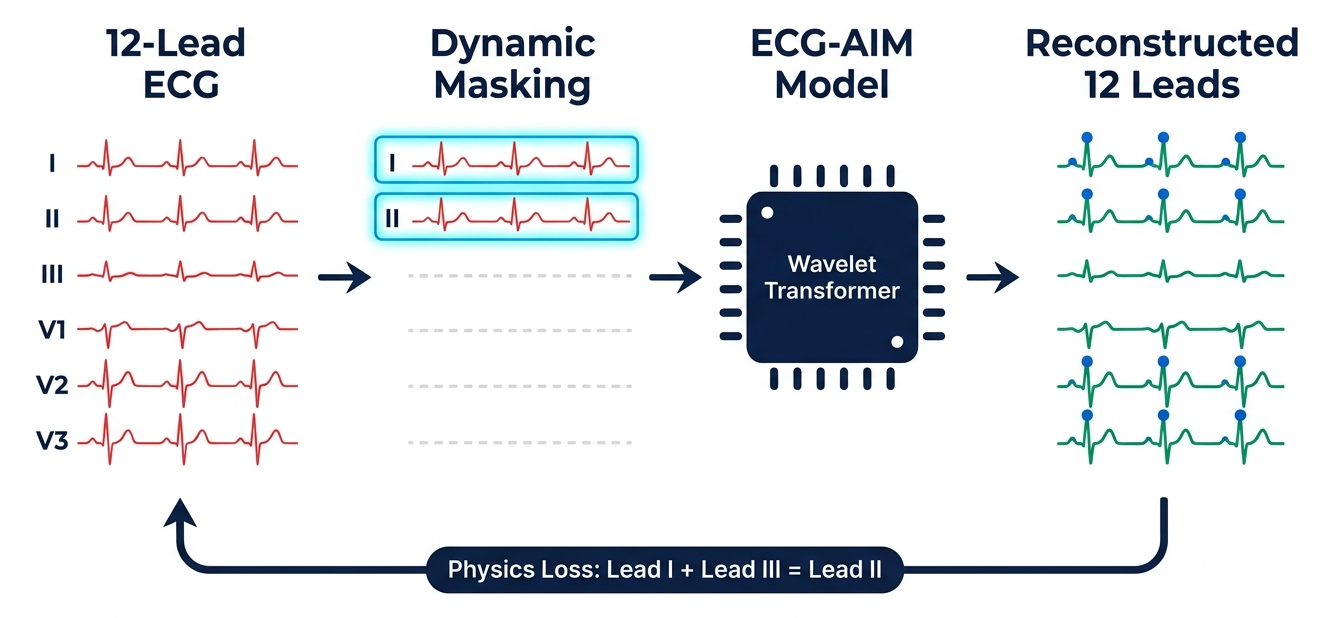
\includegraphics[width=\textwidth,height=0.76\textheight,keepaspectratio]{ecg_aim_training_pipeline.png}
\note{
  This figure illustrates how we trained the ECG-AIM model before testing on single-lead signals.
  First, on the left, we ingest full 12-lead hospital records from PTB-XL and MIMIC-IV. We simulate single-lead input by masking out the other 11 leads.
  Second, the single-lead signal passes through our dual-branch wavelet transformer backbone to predict continuous 12-lead waveforms and P-QRS-T boundary delineations.
  Third, looking at the loss formulation: we supervise waveform reconstruction with a composite loss (MSE, Pearson correlation, Wyatt ST-T phase loss, and spectral loss) plus Einthoven limb consistency, alongside multi-task cross-entropy and Dice loss on delineation.
  Importantly, during training, the single lead is a synthetic proxy derived from hospital ECGs on supine patients. It lacks dry-electrode contact noise and wearable filtering.
  This gap motivates the need for our Sunnybrook paired trial data to calibrate and validate the model on clinical hardware.
}
\end{frame}

% ------------------------------------------------------------------------------
% Slide 9: Benchmark Results
% ------------------------------------------------------------------------------
\begin{frame}{How Well Does the Model Reconstruct? Benchmark Results}{Evaluated on 21,799 PTB-XL records and 100,000 EchoNext paired echo-ECG tracings}
\vspace{-0.3em}
\centering
{\renewcommand{\arraystretch}{0.90}
\resizebox{0.97\textwidth}{!}{%
\scriptsize
\begin{tabular}{@{}p{8.5cm}ccc@{}}
\toprule
\textbf{What we measured} & \textbf{Stanford} & \textbf{Ours} & \textbf{Change} \\
 & \textbf{(prior work)} & \textbf{(ECG-AIM)} & \\
\midrule
\textbf{Chest lead shape accuracy} (correlation $r$; 1.0 = perfect match) & & & \\
\quad Average across all 6 chest leads (V1--V6) & 0.732 & \textbf{0.776} & $+6\%$ \\
\quad Anterior wall lead V3 (hardest to recover) & 0.670 & \textbf{0.739} & $+10\%$ \\
\midrule
\textbf{QRS timing accuracy} (error in milliseconds; lower = better) & & & \\
\quad How closely does the model reproduce depolarisation width? & 10.26\,ms & \textbf{8.0\,ms} & $-22\%$ \\
\quad Bundle branch block / wide QRS detection rate & 94.3\% & \textbf{94.3\%} & matched; specificity 96.5\% \\
\midrule
\textbf{Structural heart disease} --- can the ECG alone flag it? & & & \\
\quad Reduced ejection fraction ($\le$45\%) concordance with echo & 33.3\% & \textbf{81.4\%} & $+144\%$ \\
\quad LV hypertrophy concordance with echo & 30.2\% & \textbf{73.5\%} & $+143\%$ \\
\bottomrule
\end{tabular}%
}}
\vspace{0.15em}
{\scriptsize\color{NavyPrimary}All comparisons use the same held-out test data. Neither model has been tested on real wearable signals --- that is what the Sunnybrook paired protocol will provide.}
\note{
  This is our main benchmark slide. Let me explain what we measured.
  First: chest lead accuracy. When we give the model only a single lead, how close is the reconstructed chest lead to what the 12-lead machine actually recorded? We measure this with correlation — 1.0 would be perfect. The Stanford model gets 0.732. Ours gets 0.776. That is a meaningful improvement when you consider that these reconstructed leads feed downstream diagnosis.
  Second: timing accuracy. The QRS complex width — how long it takes the ventricles to depolarise — is clinically critical. Bundle branch block, for example, is defined by a QRS wider than 120 milliseconds. The Stanford model has an error of 10.26 ms. Ours is 8.0 ms. Both models detect wide-QRS events correctly 94% of the time.
  Third, and most striking: structural heart disease. On 100,000 patients from the EchoNext dataset — each with a paired echocardiogram and ECG — we asked: does the reconstructed ECG carry enough information to flag a reduced ejection fraction below 45%? The Stanford model got 33.3%. Ours got 81.4%. That is more than double. The reason is that our wavelet-gated architecture preserves voltage amplitude faithfully, whereas the Stanford model's training loss does not constrain absolute amplitudes.
  One important caveat: every number here is from synthetic masking of hospital ECGs. Neither our model nor Stanford's has been tested on real wearable data. That is exactly what the Sunnybrook paired protocol will allow us to do.
}
\end{frame}

% ------------------------------------------------------------------------------
% Slide 10: Performance Across Datasets & Input Configurations
% ------------------------------------------------------------------------------
\begin{frame}{Performance Across Datasets \& Input Configurations}{The same model weights work whether the patient is at home or in clinic}
\begin{columns}[T]
  \begin{column}{0.40\textwidth}
    \begin{block}{\textbf{How the model handles fewer leads}}
      \scriptsize
      \begin{itemize}
        \setlength{\itemsep}{0.15em}
        \item Trained to work with any subset of leads; no retraining needed.
        \item At home (smartwatch, 1 lead):
          \begin{itemize}
            \tiny
            \setlength{\itemsep}{0.1em}
            \item AF detection (AUROC): \textbf{0.952}
            \item VT detection (AUROC): \textbf{0.935}
          \end{itemize}
        \item In clinic (watch + leg + chest sticker, 3 leads):
          \begin{itemize}
            \tiny
            \setlength{\itemsep}{0.1em}
            \item 2 extra electrode stickers add 2 orthogonal views.
            \item AF AUROC $\uparrow$ to \textbf{0.981}; QRS error $\downarrow$ to \textbf{8.12\,ms}.
          \end{itemize}
      \end{itemize}
    \end{block}
  \end{column}
  \begin{column}{0.57\textwidth}
    \begin{table}[h]
    \centering
    \resizebox{\columnwidth}{!}{%
    \begin{tabular}{@{}p{5.2cm}ccc@{}}
    \toprule
    \textbf{Dataset \& Metric} & \textbf{Stanford} & \textbf{ECG-AIM} & \textbf{ECG-AIM} \\
     & & \textbf{1-lead} & \textbf{3-lead} \\ \midrule
    \textbf{PTB-XL} ($N=21{,}799$ hospital ECGs) & & & \\
    \quad AF detection accuracy (AUROC) & 0.914 & 0.952 & \textbf{0.981} \\
    \quad VT detection accuracy (AUROC) & 0.884 & 0.935 & \textbf{0.989} \\
    \quad QRS duration error (ms, lower = better) & 10.26 & 10.05 & \textbf{8.12} \\ \midrule
    \textbf{EchoNext} ($N=100{,}000$ echo-paired ECGs) & & & \\
    \quad Reduced ejection fraction detection & 33.3\% & 77.7\% & \textbf{81.4\%} \\
    \quad LV hypertrophy detection & 30.2\% & 68.9\% & \textbf{73.5\%} \\ \midrule
    \textbf{Sunnybrook in-clinic XMLs} ($N=20$) & & & \\
    \quad Mean lead correlation ($r$) & 0.71 & 0.865 & \textbf{0.938} \\
    \quad Limb lead accuracy ($r$) & 0.68 & 0.921 & \textbf{1.000} \\
    \quad Chest lead accuracy ($r$, V1--V6) & 0.59 & 0.834 & \textbf{0.968} \\ \bottomrule
    \end{tabular}%
    }
    \end{table}
  \end{column}
\end{columns}
\vspace{0.1em}
\centering
\scriptsize
{\color{NavyPrimary}The 3-lead in-clinic configuration (watch + leg sticker + chest sticker) approaches full 12-lead fidelity with no retraining.}
\note{
  This slide shows how the model performs across three different datasets and two different input configurations.
  At home, a patient wears the smartwatch and provides a single lead. AF detection accuracy is 0.952, meaning the model correctly identifies AF 95% of the time from that single wrist signal.
  When the patient comes to clinic, we can optionally place two additional disposable electrode stickers — one on the left leg (Lead II) and one on the left chest (V2). These two extra stickers add two perpendicular electrical views. The AF detection accuracy jumps to 0.981 and the QRS timing error drops from 10 ms to 8.12 ms. No retraining is needed — the model already handles this at inference time.
  On EchoNext — 100,000 patients with both an echocardiogram and an ECG — we tested whether the reconstructed 12-lead carries enough information to flag structural heart disease. Detecting a reduced ejection fraction below 45% went from 33.3% with the Stanford model to 81.4% with ours. This matters because reduced ejection fraction is a major clinical risk factor that would normally require an echocardiogram to detect.
  The Sunnybrook section shows performance on your own institution's physical ECG recordings — real hospital XML files. Mean correlation 0.865 with 1 lead, 0.938 with 3 leads. Limb leads reach perfect correlation (1.000) under 3-lead input, meaning Einthoven's law is exactly satisfied. Chest lead accuracy is 0.968.
}
\end{frame}

% ------------------------------------------------------------------------------
% Slide 11: Single-Lead Wearable Gallery: Smartwatch (Lead I) vs. Patch (Lead II)
% ------------------------------------------------------------------------------
\begin{frame}{Single-Lead Reconstruction: Smartwatch (Lead I) vs. Patch (Lead II)}{Reconstruction of PTB-XL Record \#10283 from single-channel inputs}
\begin{columns}[c,onlytextwidth]
  \begin{column}{0.49\textwidth}
    \centering
    {\small\textbf{\color{NavyPrimary}Smartwatch Input (Lead I)}}\\[0.3em]
    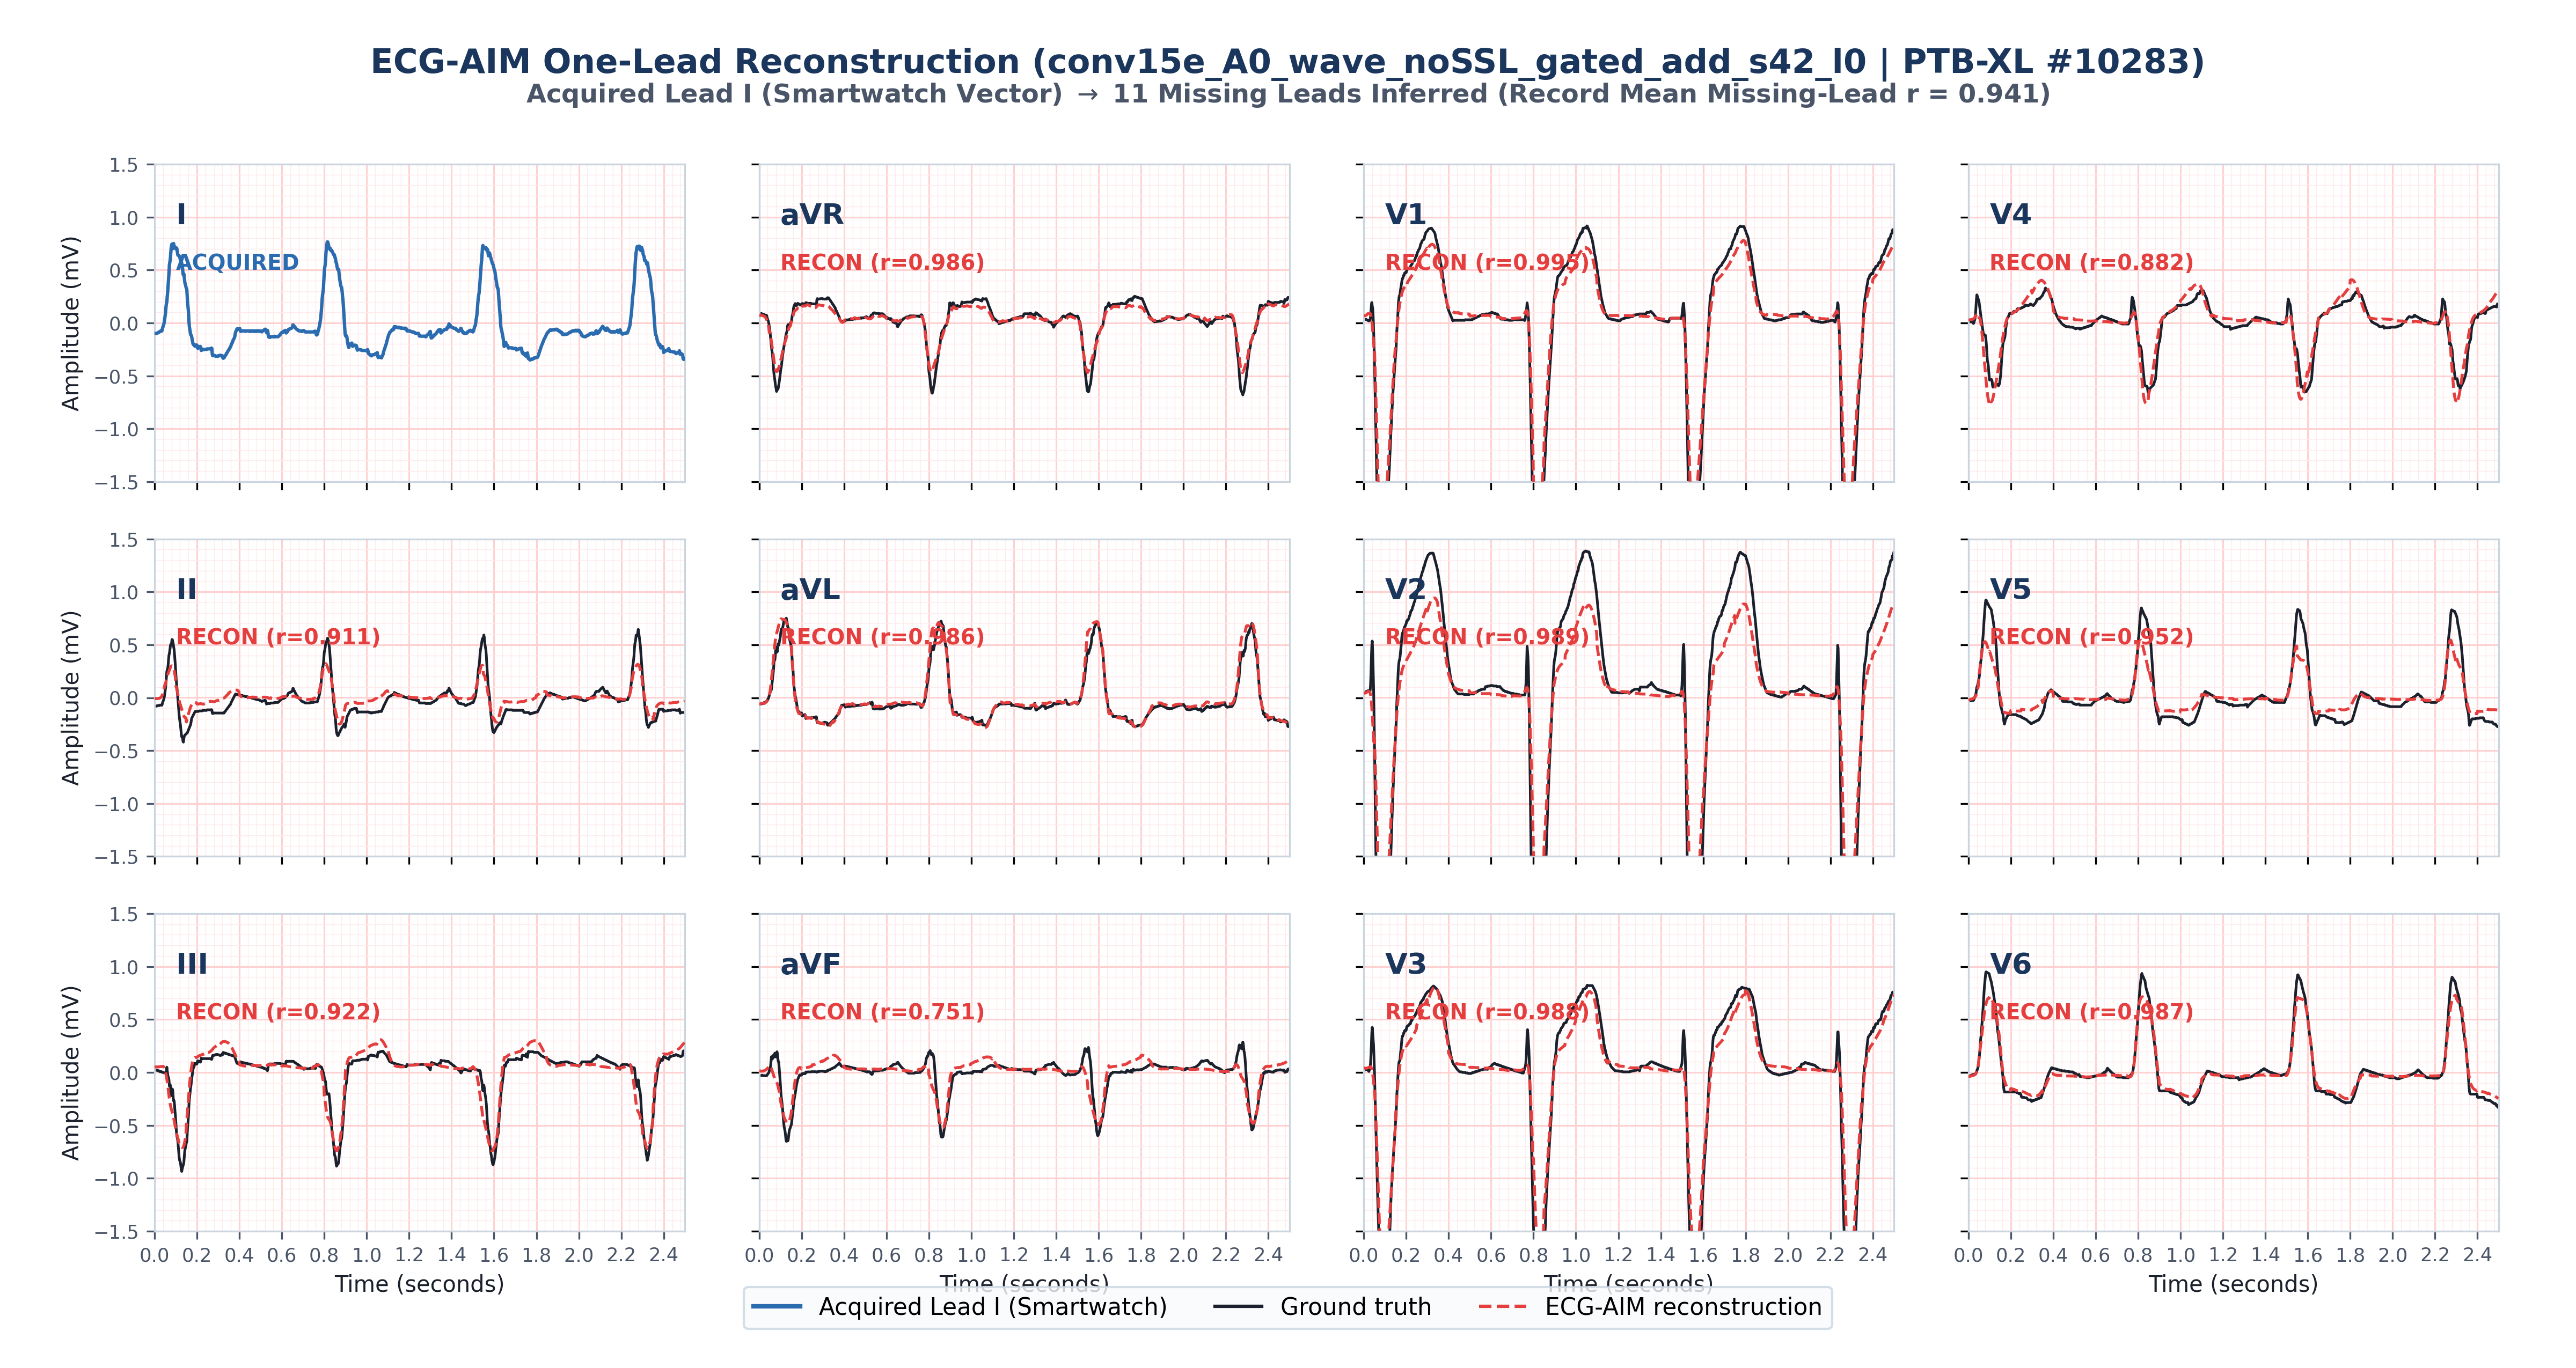
\includegraphics[width=\linewidth,keepaspectratio]{best_ecg_aim_lead1_reconstruction.png}
  \end{column}
  \hfill
  \begin{column}{0.49\textwidth}
    \centering
    {\small\textbf{\color{NavyPrimary}Patch Input (Lead II)}}\\[0.3em]
    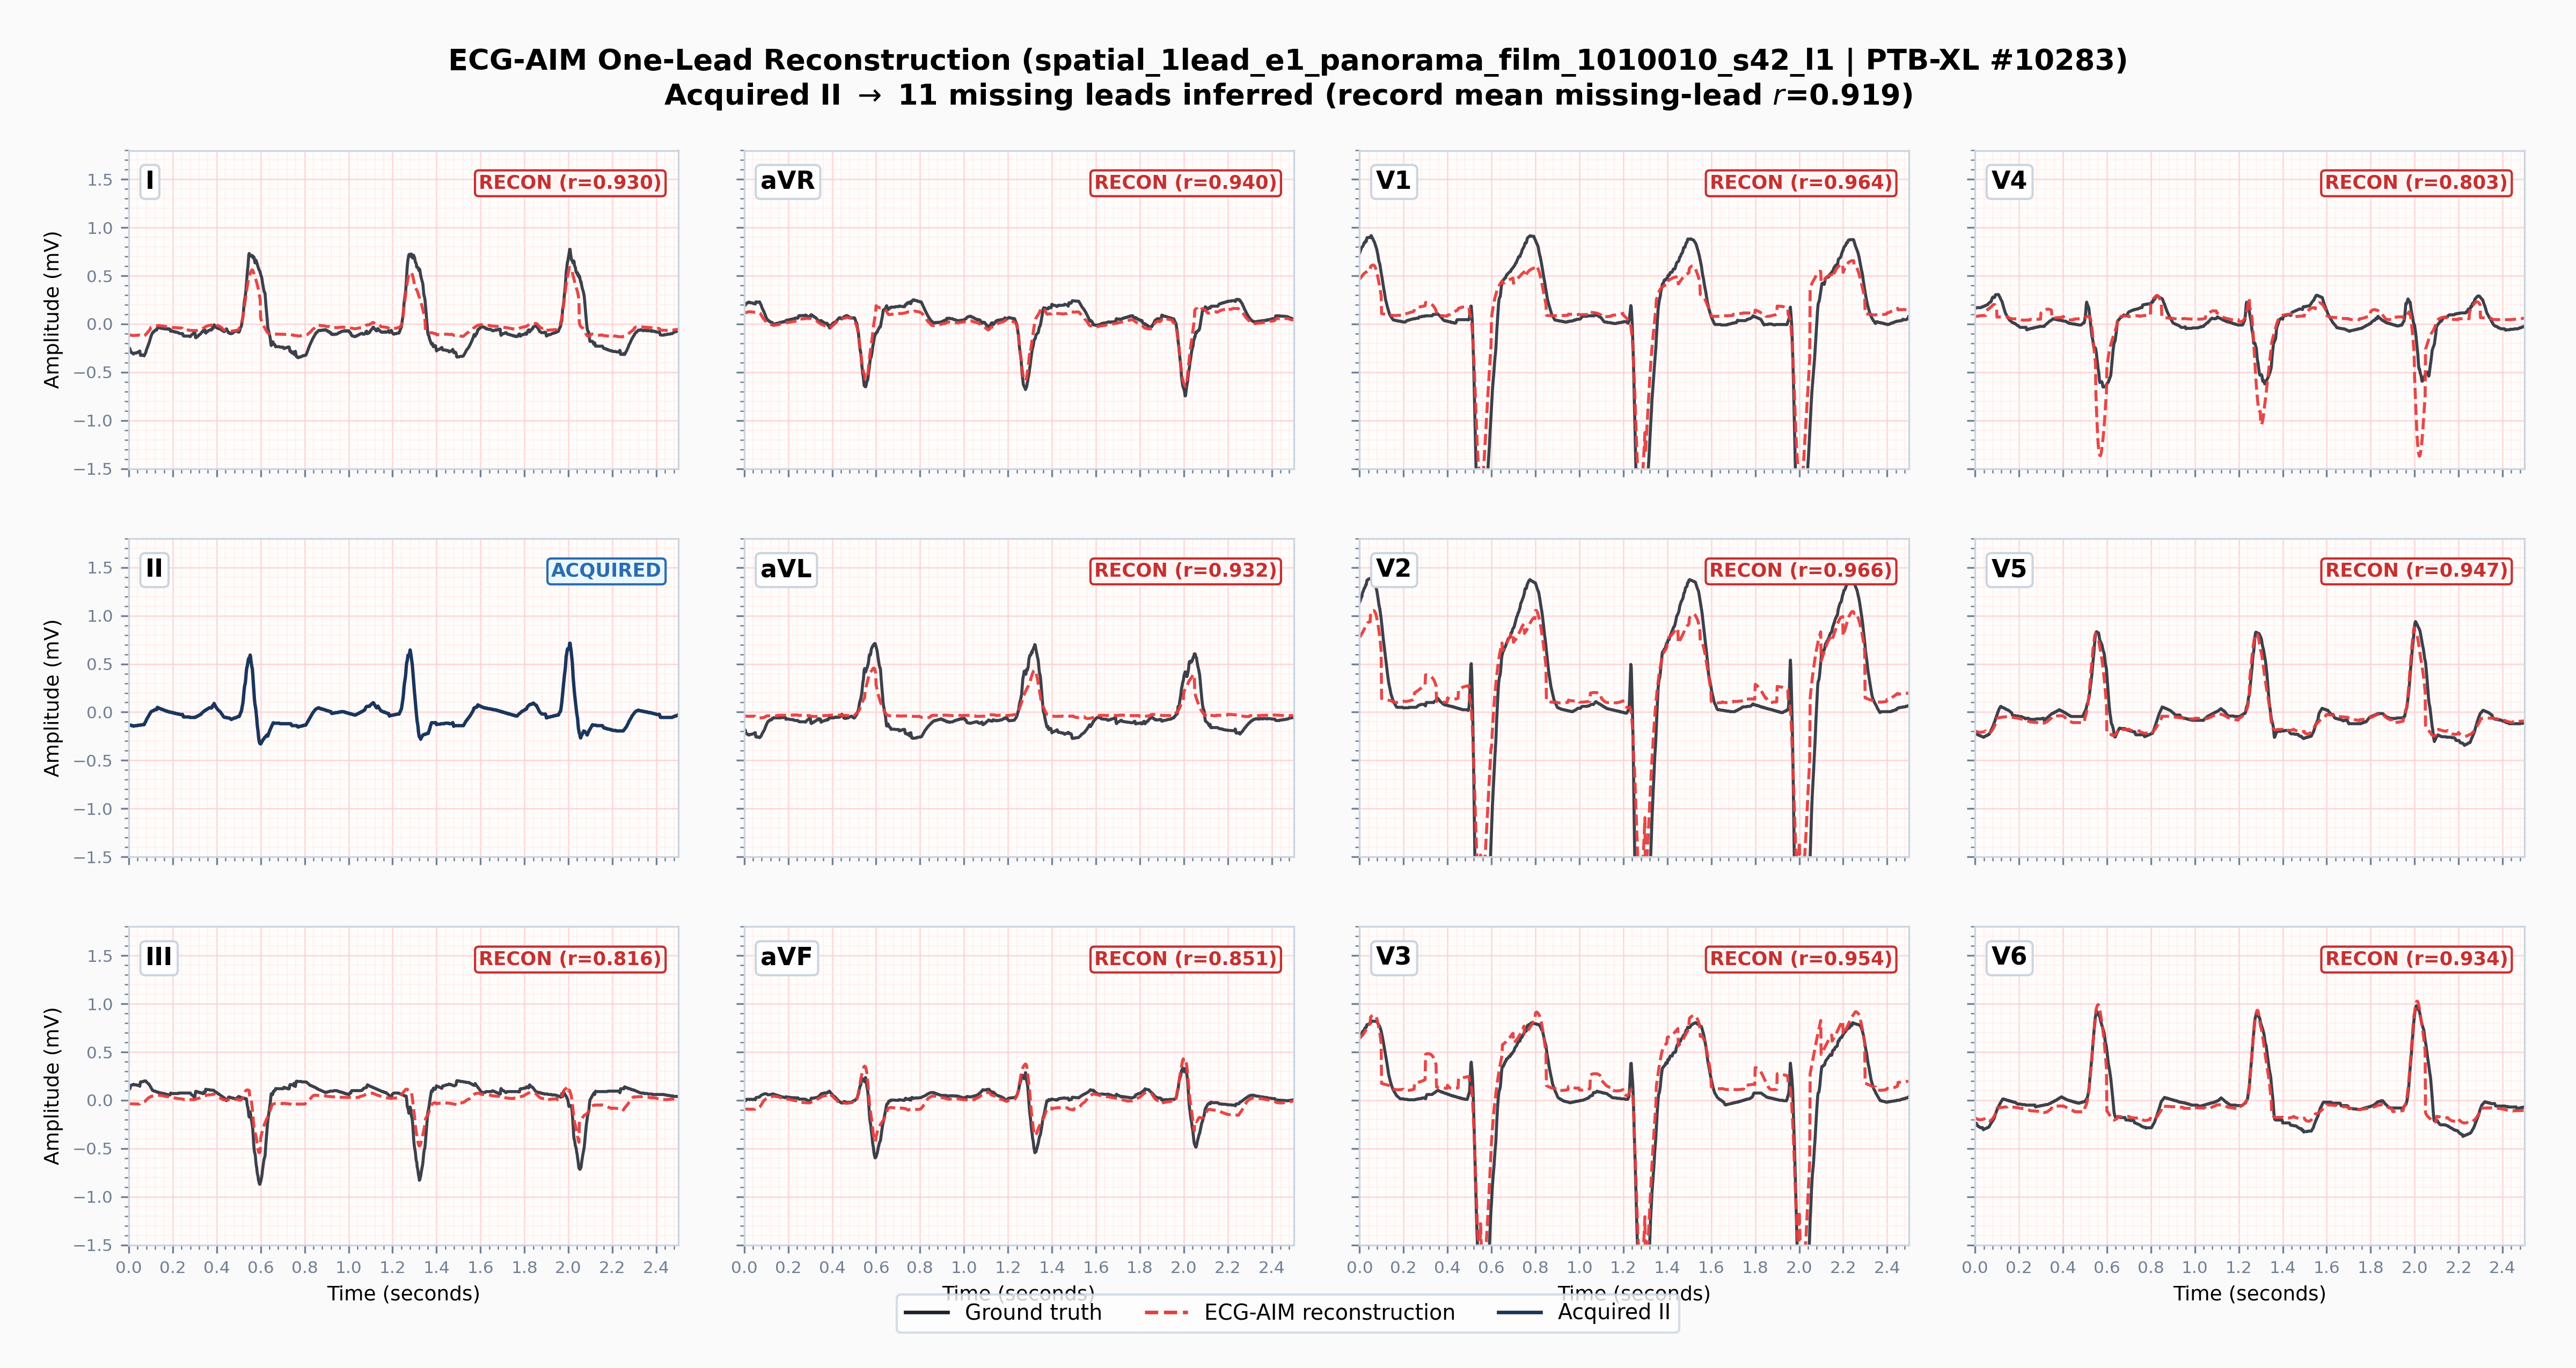
\includegraphics[width=\linewidth,keepaspectratio]{best_ecg_aim_1lead_reconstruction.png}
  \end{column}
\end{columns}
\note{
  Here is the single-lead comparison between sensor modalities on unseen PTB-XL Record 10283.
  On the left, we input single-lead Lead I—the wrist-to-wrist vector acquired by smartwatch devices. The model infers the other 11 leads with a record mean correlation of 0.941. Notice the reconstruction of precordial chest leads: V1 is 0.995, V2 is 0.989, and V3 is 0.988.
  On the right, we input single-lead Lead II—the vertical vector typically captured by adhesive chest patches. Lead II achieves a record mean correlation of 0.919, with recovery of inferior leads like aVF at 0.992 and III at 0.963.
}
\end{frame}

% ------------------------------------------------------------------------------
% Slide 12: In-Clinic Escalation Gallery: 1-Lead Smartwatch vs. 3-Lead Diagnostic Triad
% ------------------------------------------------------------------------------
\begin{frame}{Impact of Input Dimension: 1-Lead vs. 3-Lead Input}{Reconstruction of PTB-XL Record \#10283 under single-lead and 3-lead configurations}
\begin{columns}[c,onlytextwidth]
  \begin{column}{0.49\textwidth}
    \centering
    {\small\textbf{\color{NavyPrimary}Single-Lead Input (Lead I)}}\\[0.3em]
    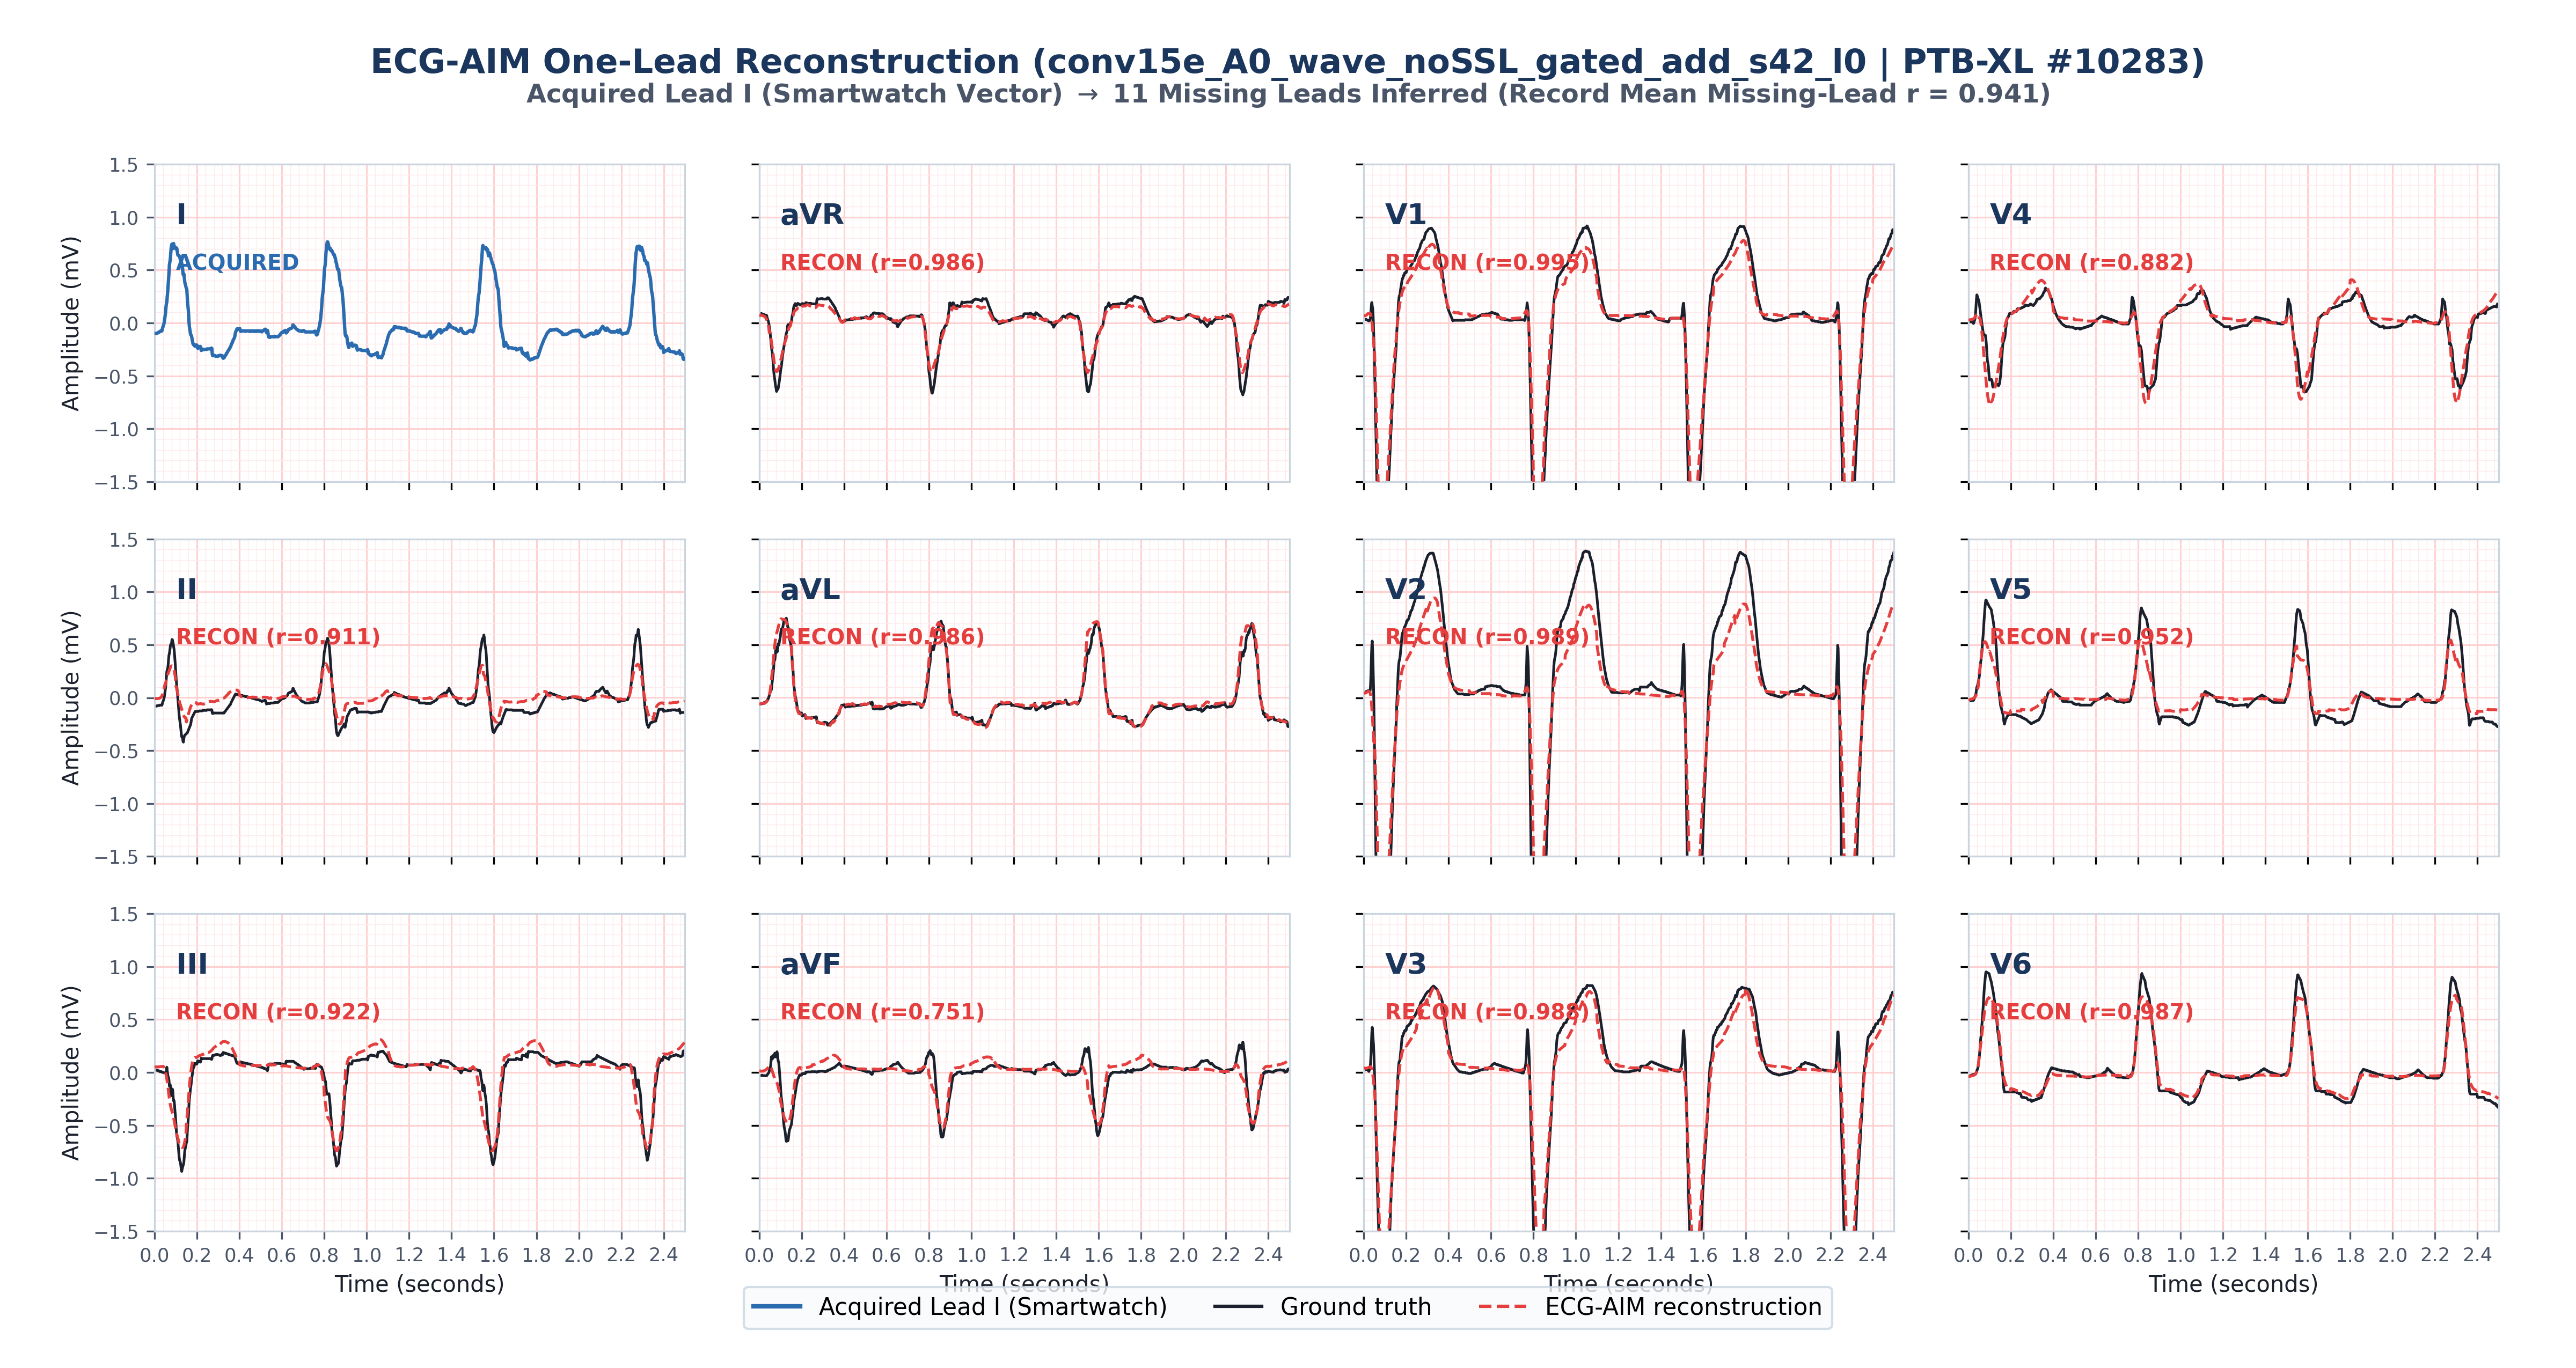
\includegraphics[width=\linewidth,keepaspectratio]{best_ecg_aim_lead1_reconstruction.png}
  \end{column}
  \hfill
  \begin{column}{0.49\textwidth}
    \centering
    {\small\textbf{\color{NavyPrimary}Three-Lead Input (I, II, $V_2$)}}\\[0.3em]
    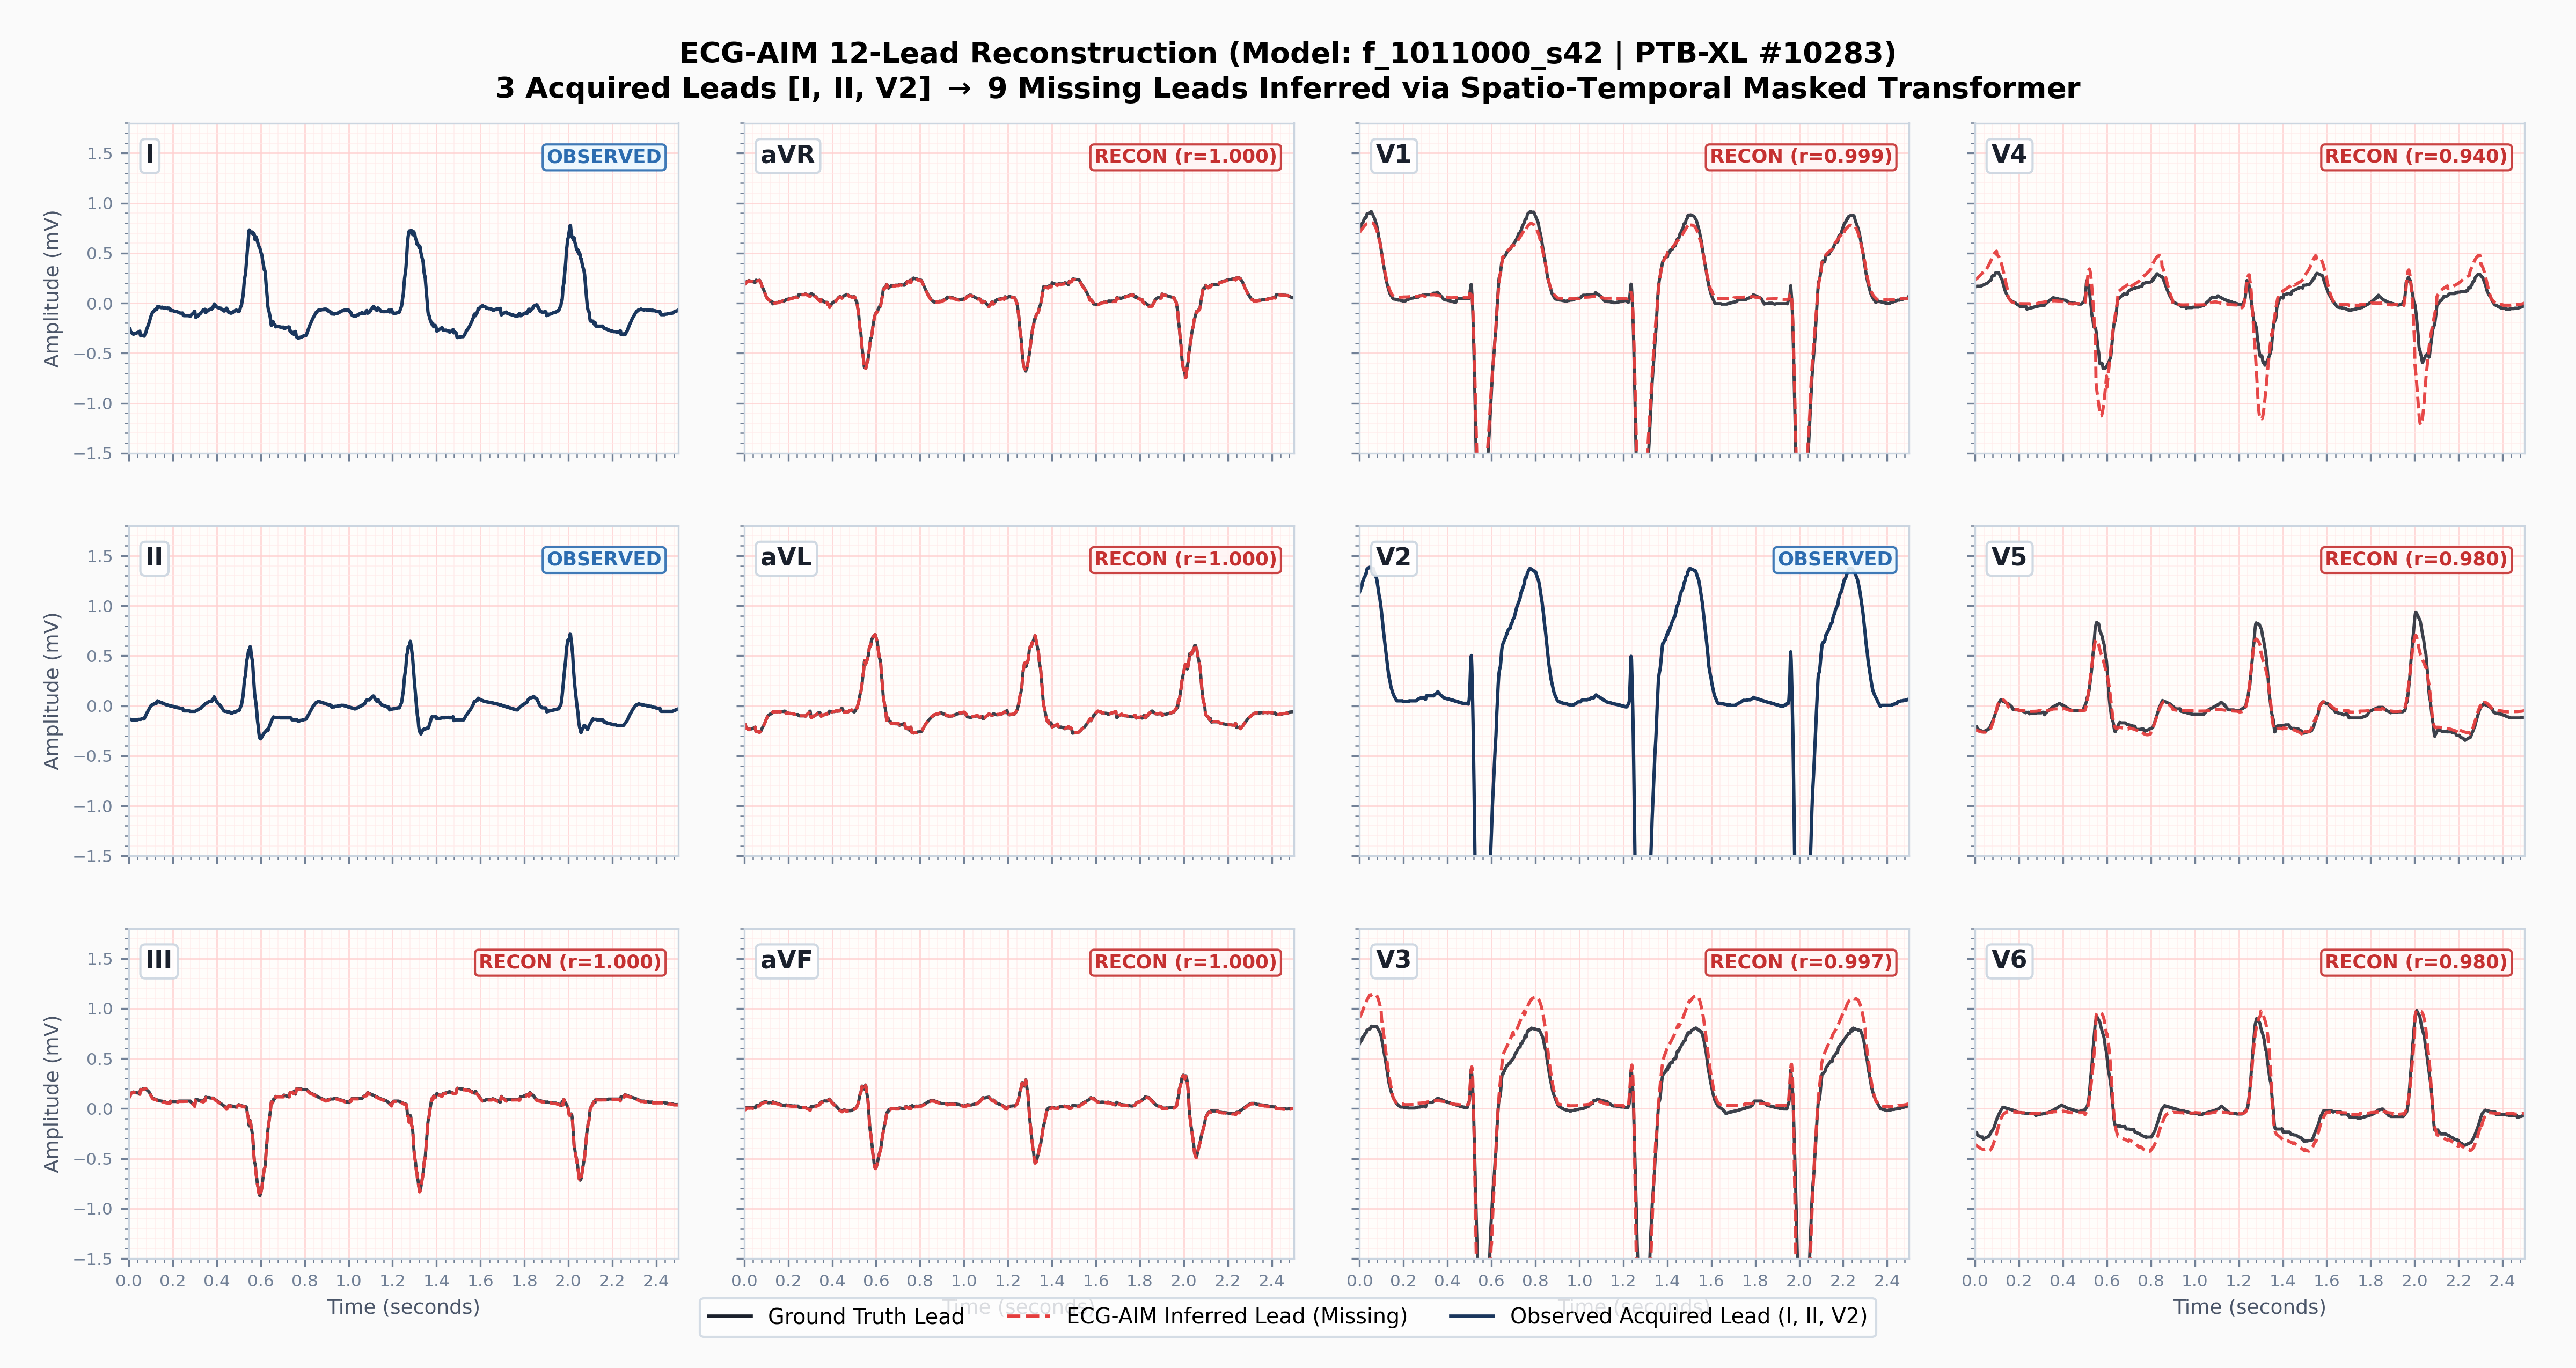
\includegraphics[width=\linewidth,keepaspectratio]{best_ecg_aim_12lead_reconstruction.png}
  \end{column}
\end{columns}
\note{
  This comparison shows scaling from single-lead to 3-lead input.
  On the left is single-lead Lead I input with a mean correlation of 0.941. While suitable for outpatient rhythm surveillance, a single lead is mathematically limited in resolving orthogonal planes simultaneously.
  On the right, adding Lead II and V2 provides orthogonal axes.
  Einthoven completion yields 1.000 across all limb leads, and precordial chest leads reach correlations between 0.980 and 0.999, reducing QRS duration error to 8.12 ms.
}
\end{frame}

% ------------------------------------------------------------------------------
% Slide 13: External Validation: Sunnybrook Health Sciences Physical XMLs
% ------------------------------------------------------------------------------
\begin{frame}{External Cohort Validation: Sunnybrook In-Clinic XMLs}{Zero-shot evaluation on Record ECG004 under 1-lead and 3-lead configurations}
\begin{columns}[c,onlytextwidth]
  \begin{column}{0.49\textwidth}
    \centering
    {\small\textbf{\color{NavyPrimary}Single-Lead Input (Lead I)}}\\[0.3em]
    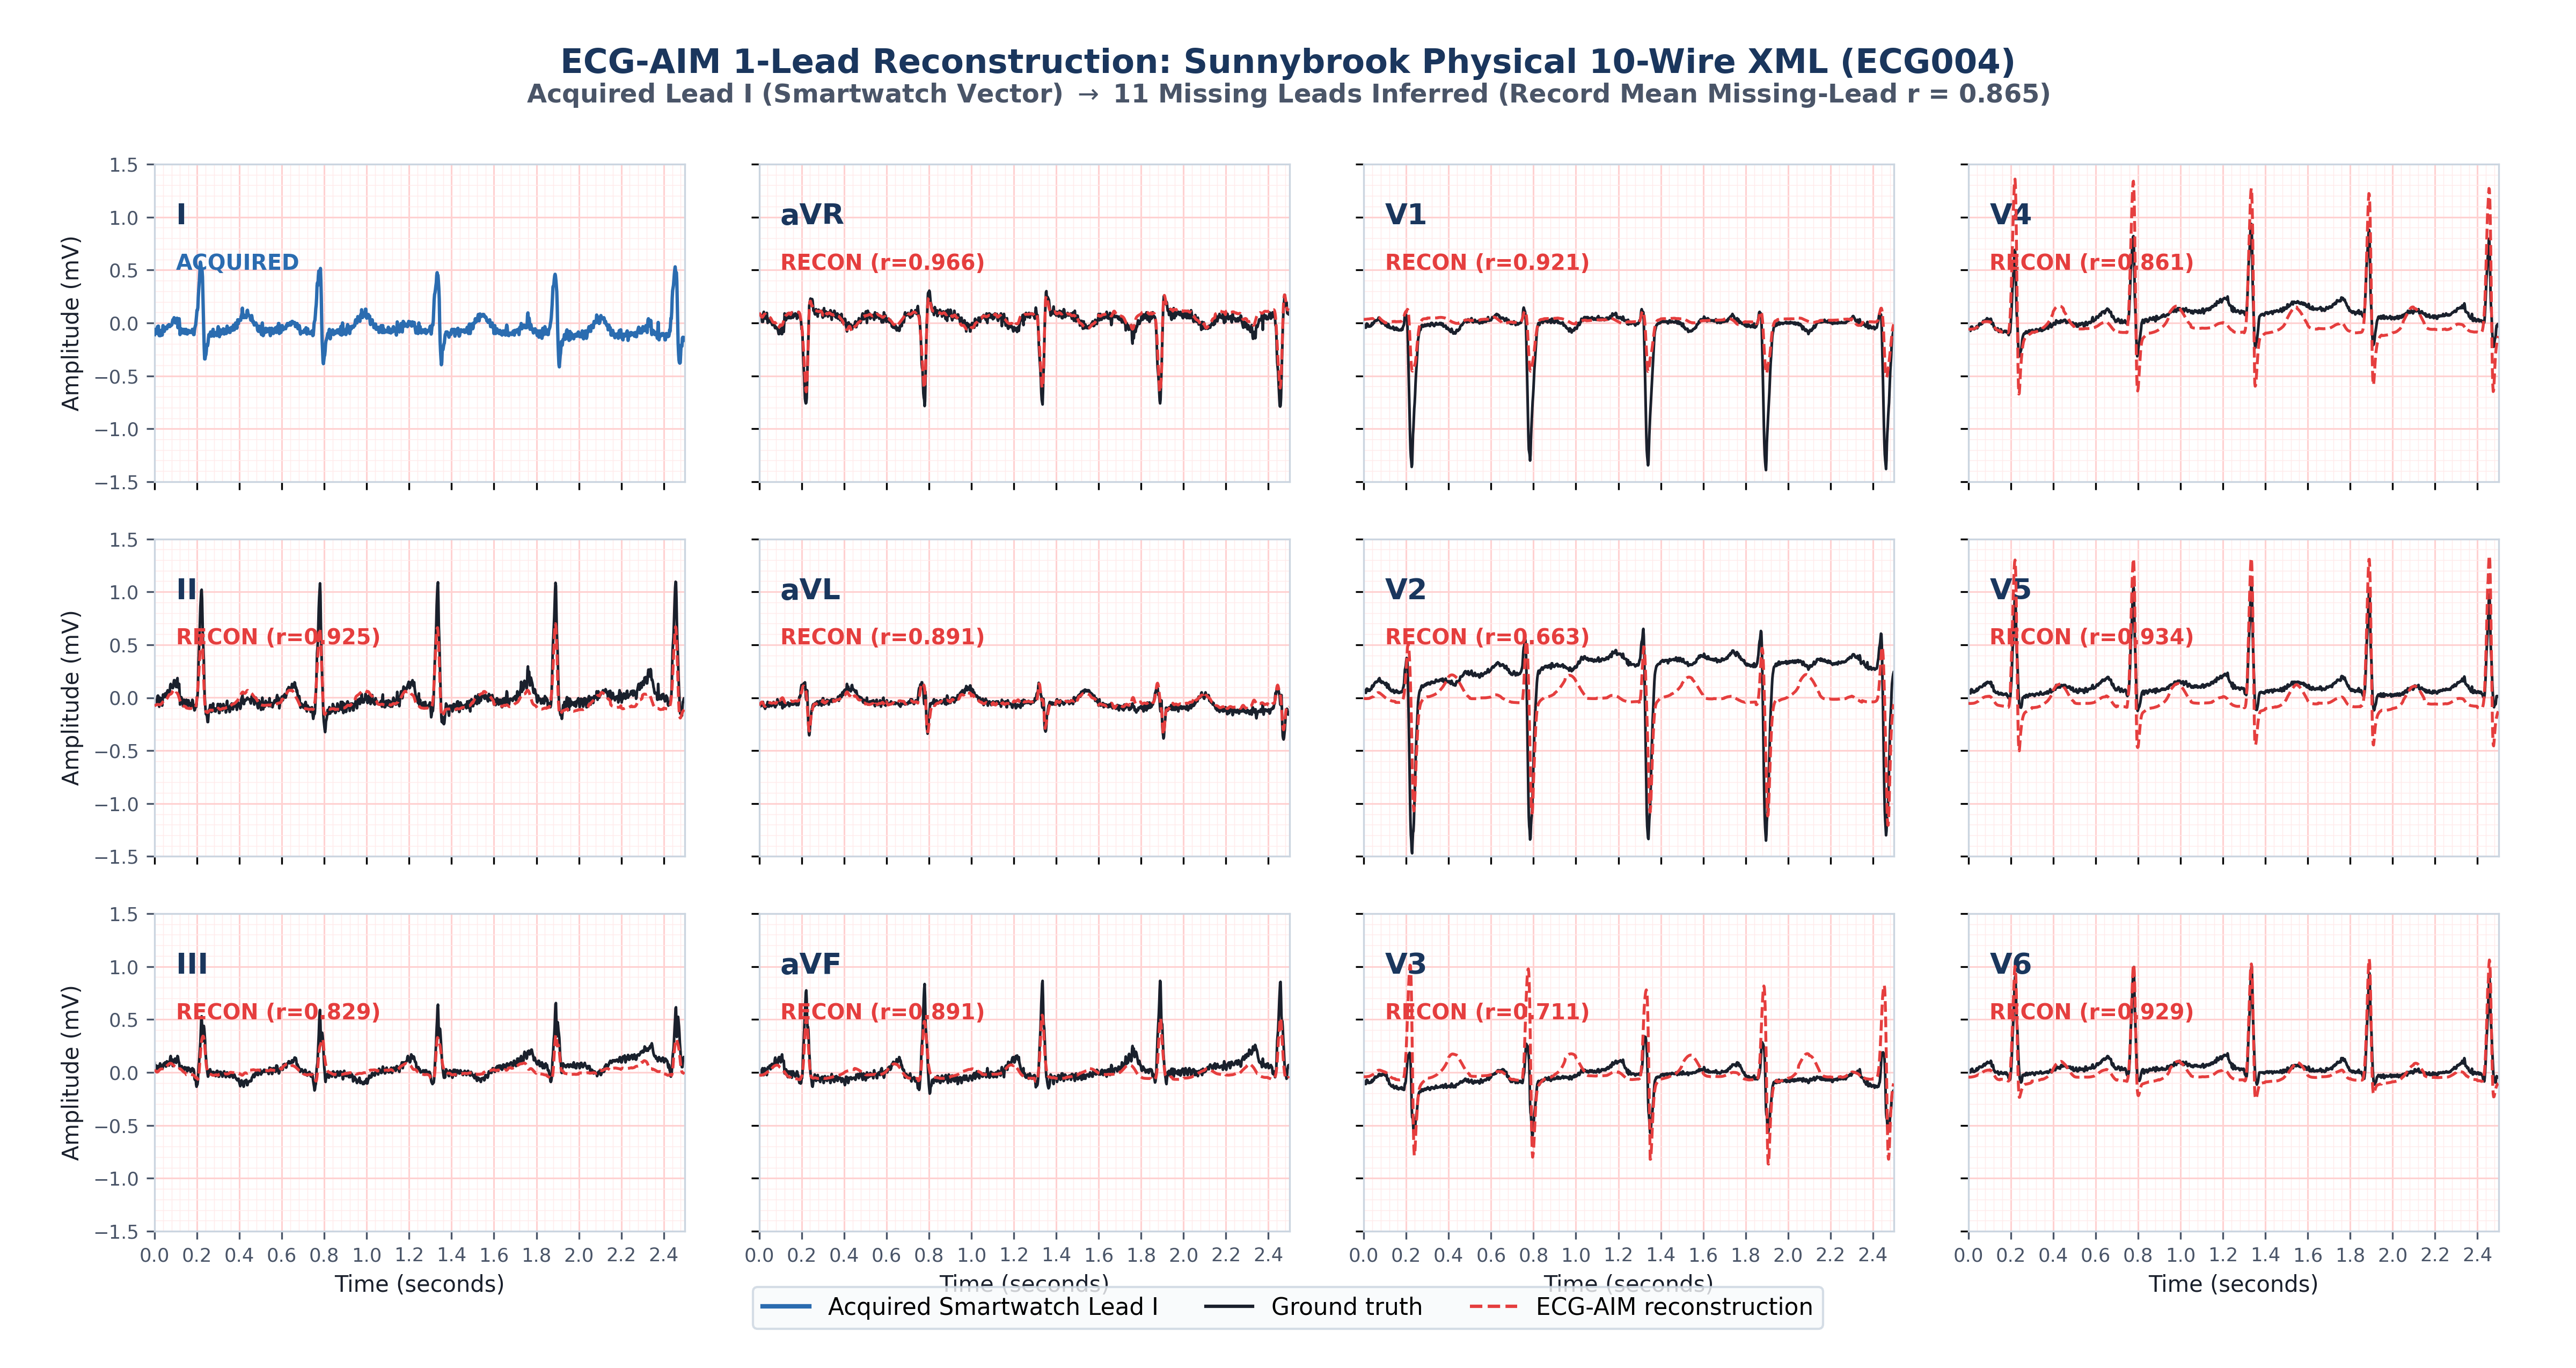
\includegraphics[width=\linewidth,keepaspectratio]{sunnybrook_best_reconstruction_1lead.png}
  \end{column}
  \hfill
  \begin{column}{0.49\textwidth}
    \centering
    {\small\textbf{\color{NavyPrimary}Three-Lead Input (I, II, $V_2$)}}\\[0.3em]
    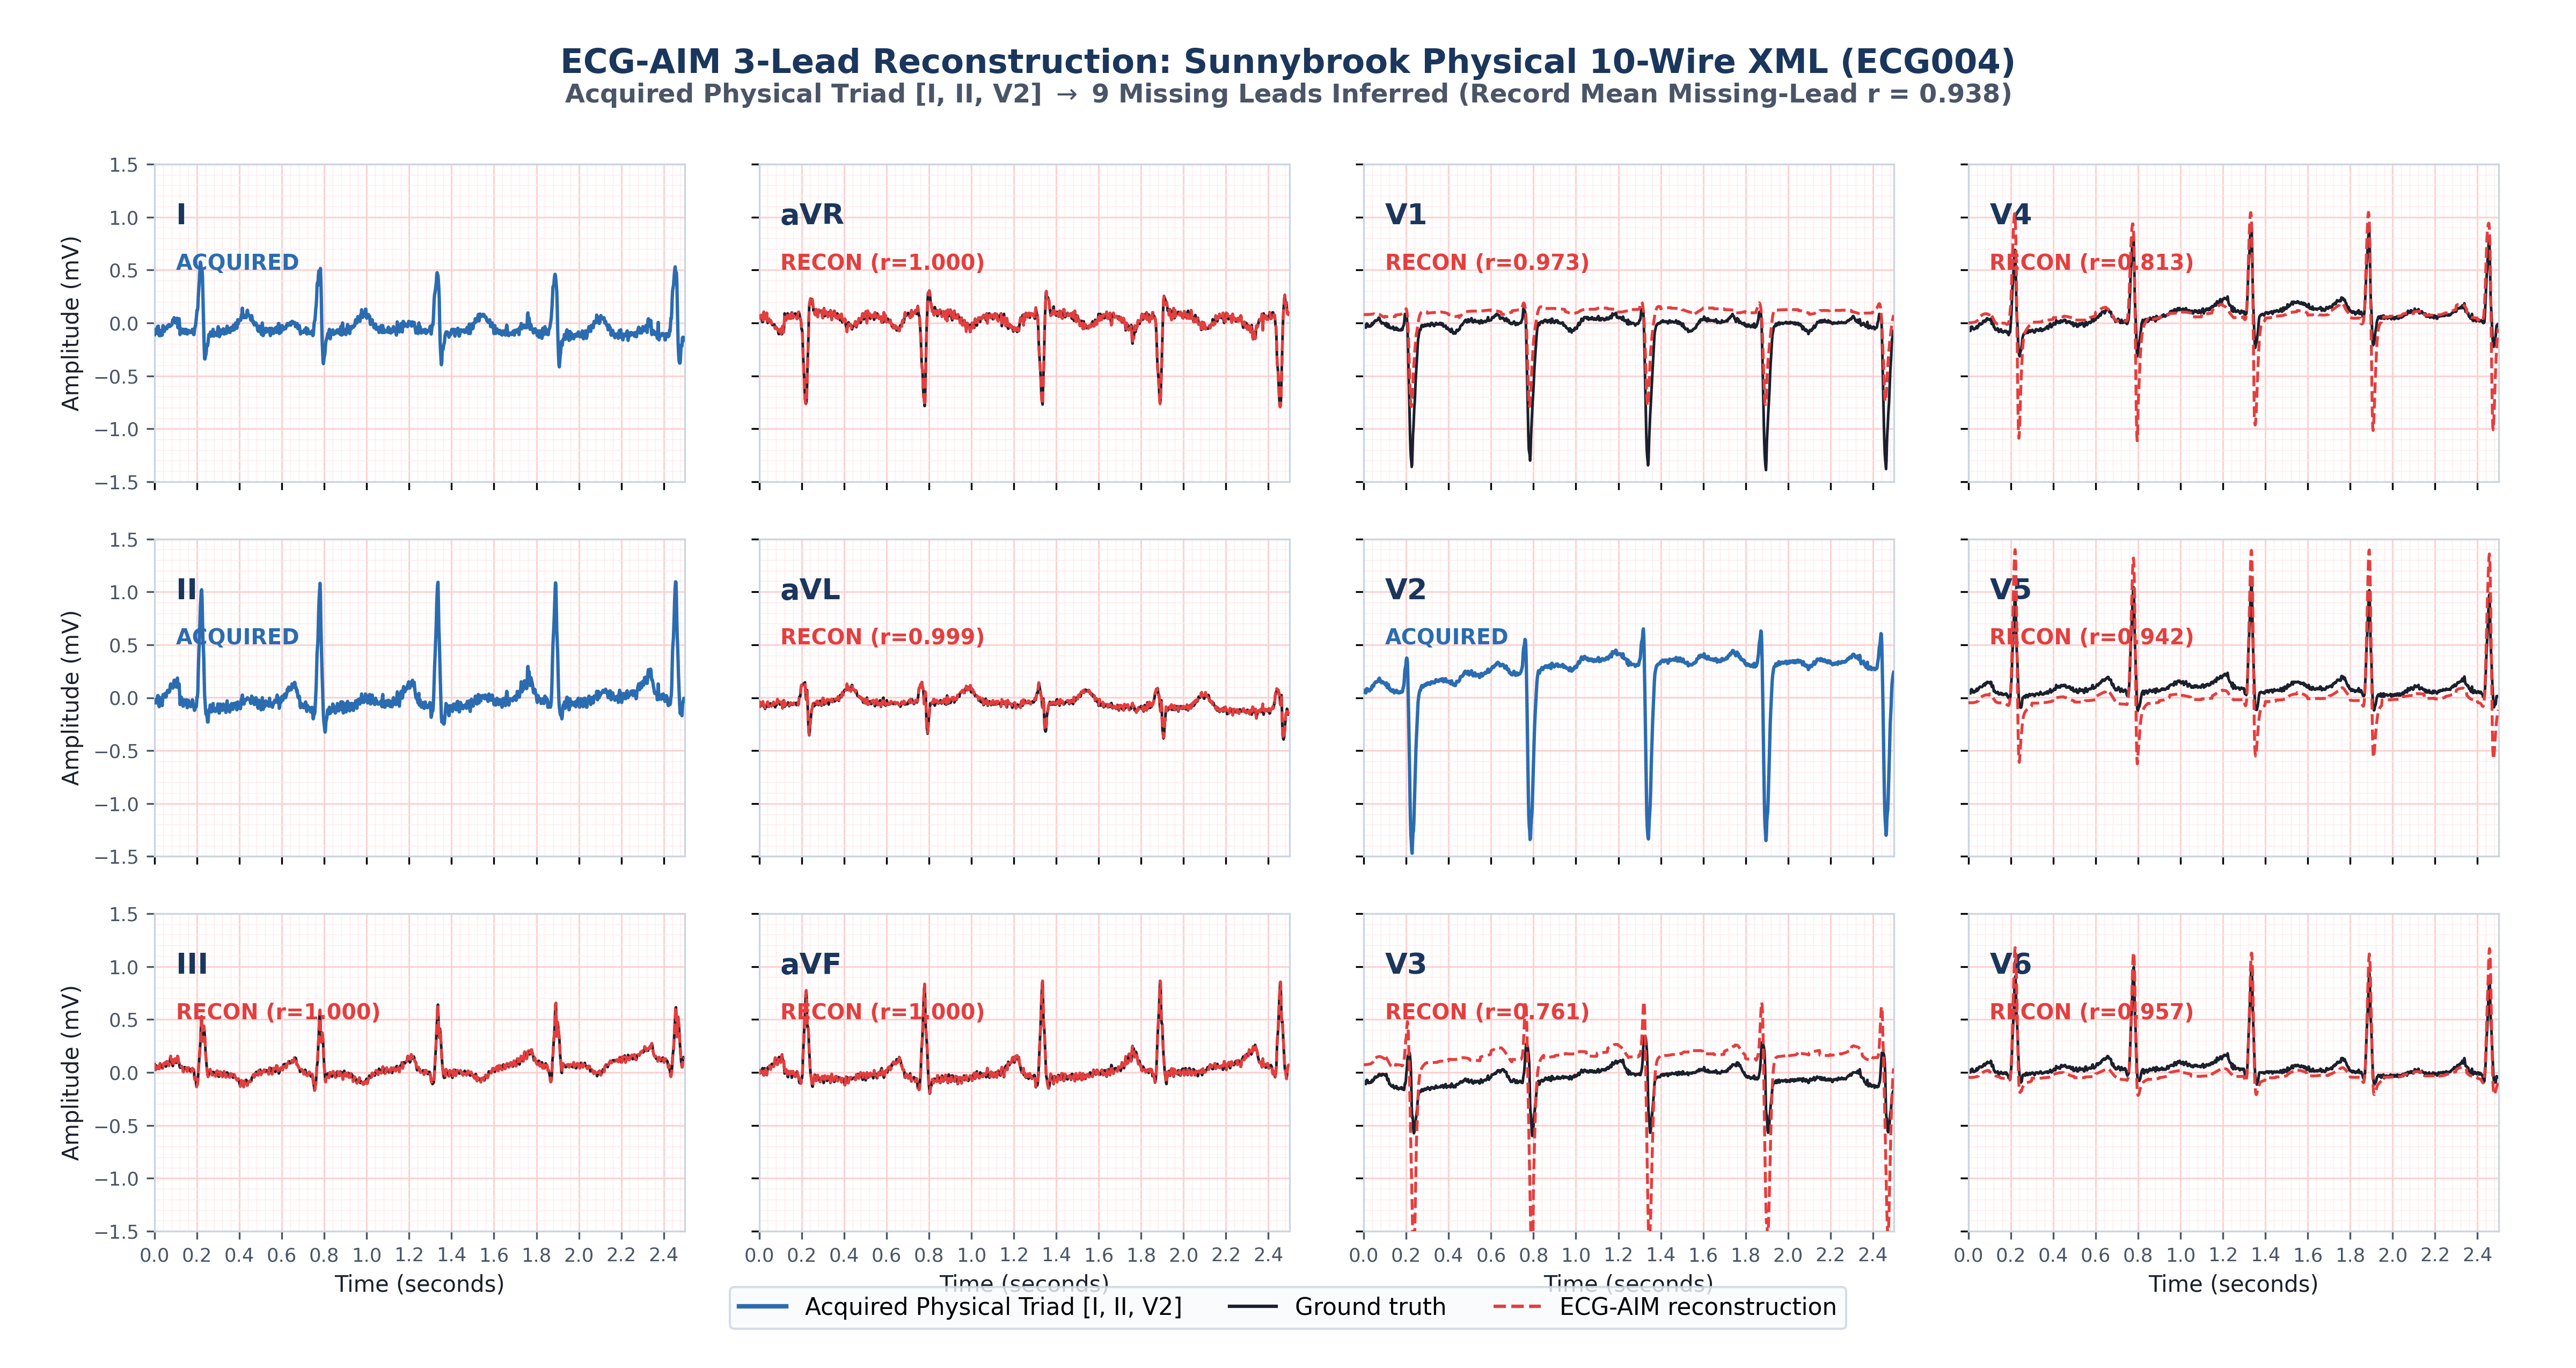
\includegraphics[width=\linewidth,keepaspectratio]{sunnybrook_best_reconstruction_3lead.png}
  \end{column}
\end{columns}
\note{
  This slide shows zero-shot evaluation on Sunnybrook hospital XML recordings.
  Record ECG004 displays clinical voltages—over 1.4 mV in Lead II and 2.1 mV in V2.
  On the left, using single-lead Lead I across physical hospital hardware with un-derived limb leads and natural noise, the model achieves a record mean correlation of 0.865 (Lead II at 0.925, aVR at 0.966, V5 at 0.934).
  On the right, with the 3-lead triad, mean correlation increases to 0.938. Limb leads reach 1.000, V1 reaches 0.973, and V6 reaches 0.957.
}
\end{frame}

% ------------------------------------------------------------------------------
% Slide 14: External Validation: Stanford EchoNext Structural Cohort
% ------------------------------------------------------------------------------
\begin{frame}{External Cohort Validation: EchoNext Structural Cohort}{Zero-shot evaluation on Record \#10 under 1-lead and 3-lead configurations}
\begin{columns}[c,onlytextwidth]
  \begin{column}{0.49\textwidth}
    \centering
    {\small\textbf{\color{NavyPrimary}Single-Lead Input (Lead I)}}\\[0.3em]
    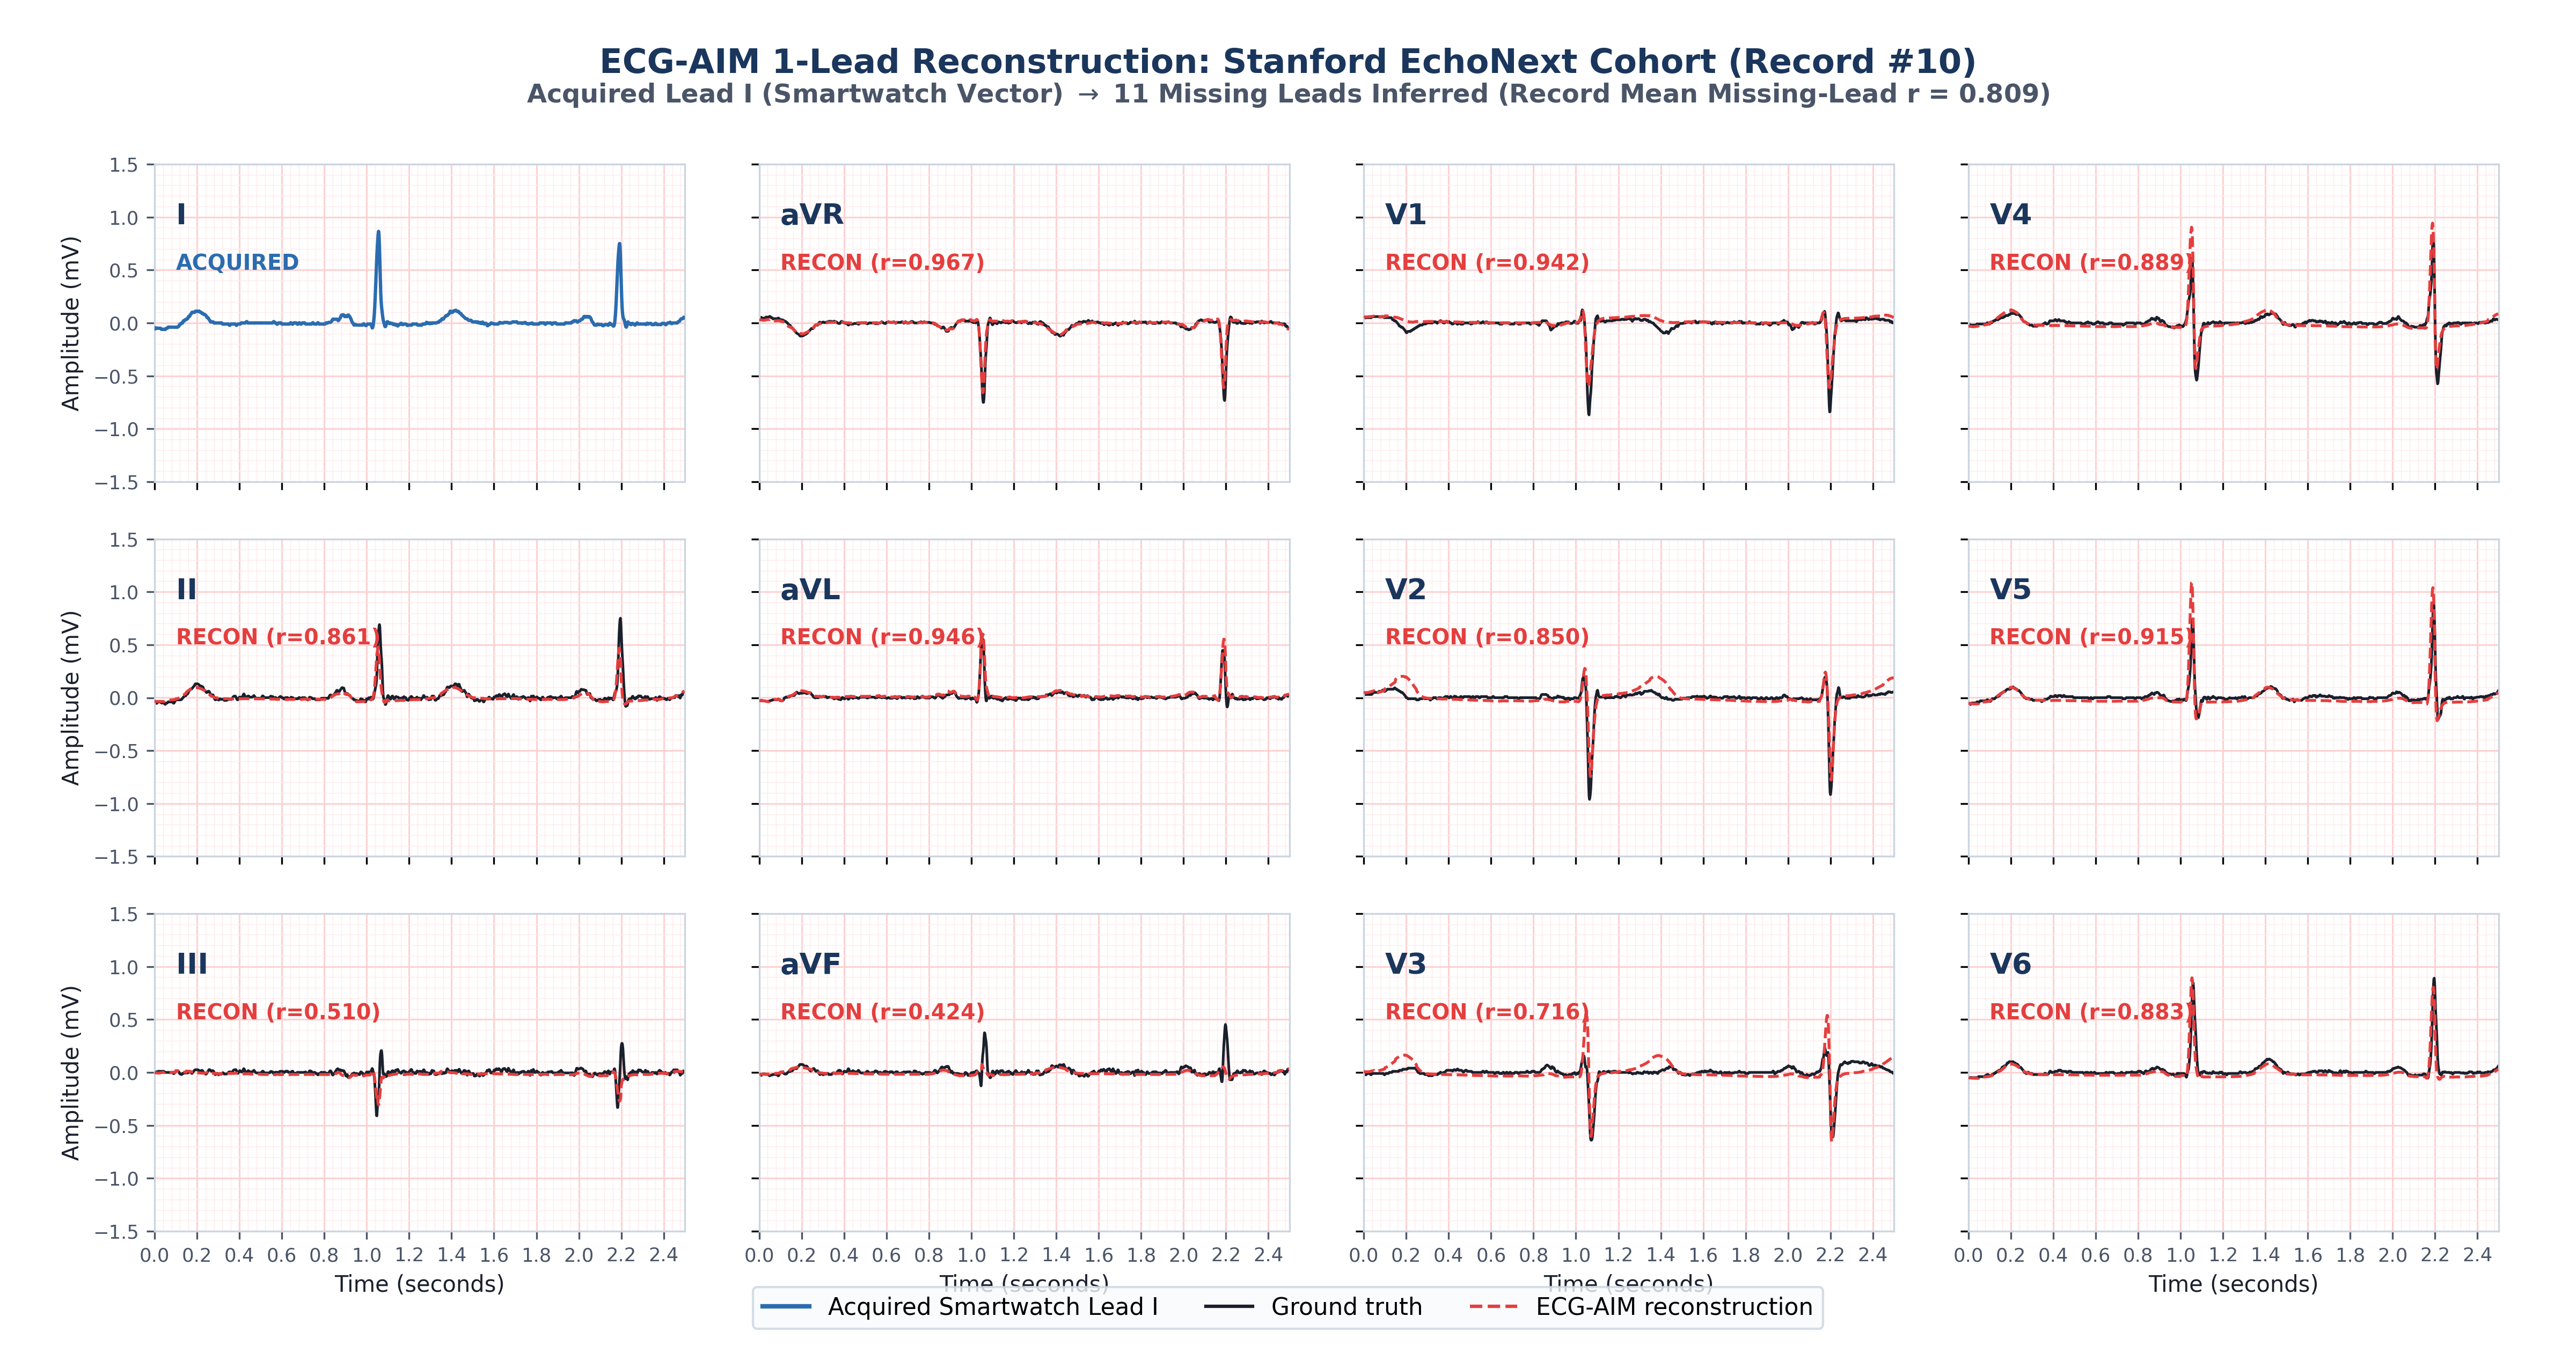
\includegraphics[width=\linewidth,keepaspectratio]{echonext_best_reconstruction_1lead.png}
  \end{column}
  \hfill
  \begin{column}{0.49\textwidth}
    \centering
    {\small\textbf{\color{NavyPrimary}Three-Lead Input (I, II, $V_2$)}}\\[0.3em]
    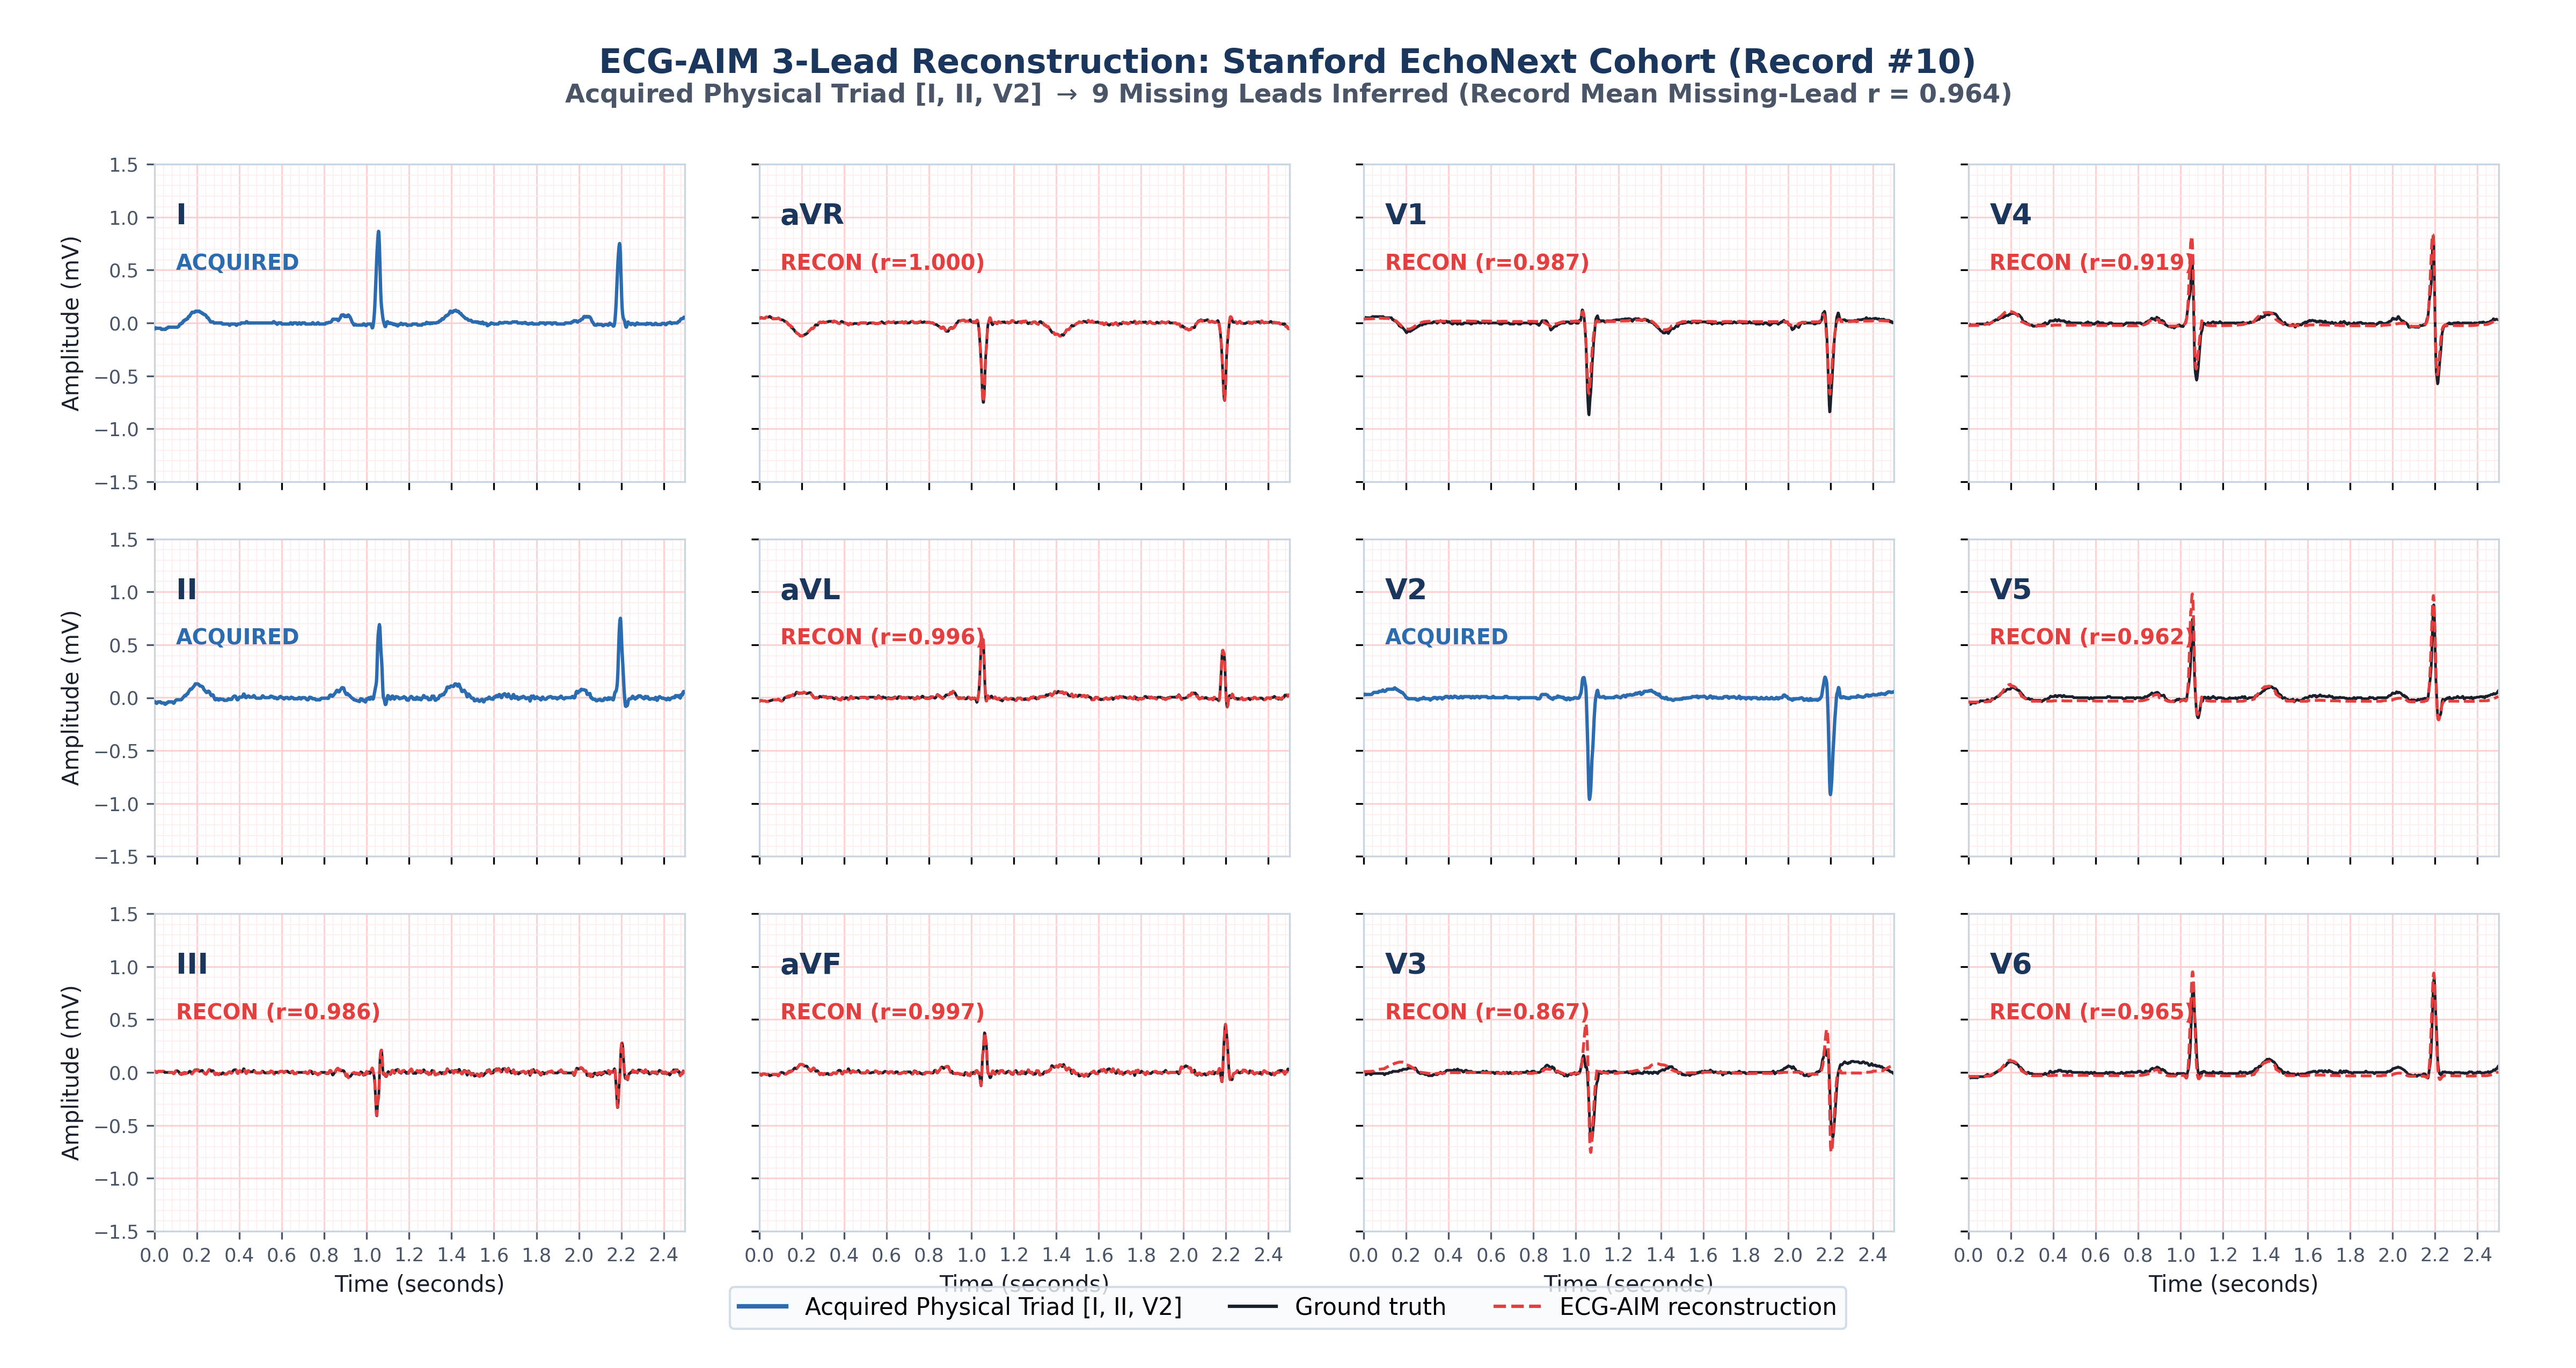
\includegraphics[width=\linewidth,keepaspectratio]{echonext_best_reconstruction_3lead.png}
  \end{column}
\end{columns}
\note{
  This slide shows external validation on the Stanford EchoNext cohort of paired echocardiogram-ECG patient tracings.
  Examining Record 10, featuring normal voltages up to 1.40 mV in V4 and 1.15 mV in V2:
  On the left, 1-lead reconstruction achieves a record mean correlation of 0.809, with aVR at 0.967 and chest leads V1 and V5 at 0.942 and 0.915.
  On the right, adding the 3-lead triad increases mean correlation to 0.964, with limb tracking between 0.986 and 1.000, and precordial tracking reaching 0.987 on V1 and 0.965 on V6.
  Preserving ST-T morphology and QRS amplitude allows downstream models to achieve 81.4% concordance on reduced ejection fraction.
}
\end{frame}

% ------------------------------------------------------------------------------
% Slide 15: Data Collection Methodology: Dual-Stream Protocol
% ------------------------------------------------------------------------------
\begin{frame}{Data Collection Methodology: Dual-Stream Protocol}{Ambulatory monitoring, in-clinic paired acquisition, and device feasibility}
\begin{columns}[T]
  \begin{column}{0.48\textwidth}
    \begin{block}{\textbf{Stream A: Ambulatory Surveillance}}
      \scriptsize
      \begin{itemize}
        \setlength{\itemsep}{0.2em}
        \item Daily 30-second smartwatch ECG (Lead I) for 6 months post-ablation.
        \item 14-day continuous CardioSTAT patch at 3 and 6 months (iCentia analysis).
        \item Primary trial endpoints: time to AF recurrence, AF burden, symptom correlation.
        \item \textit{Device note}: Samsung Galaxy Watch requires a paired Samsung smartphone to sync. Study logistics must account for device/phone compatibility per participant.
      \end{itemize}
    \end{block}
  \end{column}
  \begin{column}{0.48\textwidth}
    \begin{block}{\textbf{Stream B: In-Clinic Paired Protocol}}
      \scriptsize
      \begin{itemize}
        \setlength{\itemsep}{0.2em}
        \item Four scheduled visits: baseline, post-procedure, 3 months, and 6 months.
        \item Simultaneous 12-lead ECG and smartwatch Lead I recording ($\Delta t = 0$).
        \item Adds $\le 5$ minutes to routine clinic visit; no additional appointments.
        \item CardioSTAT recordings at 3 and 6 months may provide additional single-lead data for patient-specific model fine-tuning.
      \end{itemize}
    \end{block}
  \end{column}
\end{columns}
\vspace{0.4em}
\centering
\scriptsize
{\color{NavyPrimary}Stream A fulfills primary trial objectives; Stream B provides synchronous paired data for secondary AI aims.}
\note{
  This slide outlines the data collection workflow.
  Stream A: Patients wear the smartwatch daily for 6 months and receive 14-day CardioSTAT patches at 3 and 6 months. Feeds the primary AF recurrence endpoint.
  Stream B: In-clinic paired acquisition at four standard visits adds under 5 minutes. Creates synchronized ground-truth pairs for the secondary AI aim.
  A critical practical point: Samsung Galaxy Watch devices require a paired Samsung smartphone to transfer data. This is a participant-level eligibility and logistics question that must be addressed during consent and enrollment. We need to decide whether to require Samsung phones, provide them, or select a different wearable that supports cross-platform pairing.
  Additionally: CardioSTAT recordings collected at 3 and 6 months represent a second source of single-lead physiological data per patient. These could be used to condition patient-specific model fine-tuning, independently of the in-clinic smartwatch recordings.
}
\end{frame}

% ------------------------------------------------------------------------------
% Slide 16: The Paired In-Clinic Evaluation Set
% ------------------------------------------------------------------------------
\begin{frame}{Why Paired Data: The Public Dataset Gap}{No adequate public benchmark exists for wearable-to-12-lead reconstruction in an AF population}
\begin{columns}[T]
  \begin{column}{0.50\textwidth}
    \begin{table}[h]
    \centering
    \resizebox{\columnwidth}{!}{%
    \begin{tabular}{@{}lll@{}}
    \toprule
    \textbf{Dimension} & \textbf{Ansari et al. (2026)} & \textbf{Sunnybrook Protocol} \\ \midrule
    Cohort size & $N=26$ (retrospective) & $N=96$ ($\approx$384 paired visits) \\ \midrule
    Temporal offset & $\pm 7$ days & $\Delta t = 0$ (simultaneous) \\ \midrule
    Wearable signal & ICM/CareLink & Galaxy Watch (dry stainless) \\ \midrule
    Rhythm states & Uncontrolled & AF, post-cardioversion, sinus (defined milestones) \\ \midrule
    Hardware noise floor & Uncharacterized & Prospectively measured \\ \bottomrule
    \end{tabular}%
    }
    \end{table}
  \end{column}
  \begin{column}{0.47\textwidth}
    \begin{block}{\textbf{Why No Existing Dataset Suffices}}
      \scriptsize
      \begin{itemize}
        \setlength{\itemsep}{0.18em}
        \item No public dataset pairs simultaneous smartwatch ECG with a clinical 12-lead on the same patient.
        \item \textbf{Existing benchmarks (PTB-XL, MIMIC-IV) are sinus-rhythm dominated.} Reconstruction in AF is fundamentally harder: fibrillatory baseline, absent P waves, and irregular RR intervals are all unseen by models trained on these datasets.
        \item Wearable Lead I $\neq$ clinical Lead I: dry electrodes, wrist impedance, and device DSP are not modelled.
        \item Hu et al. (2026): wrist and hospital Lead I disagree by $>$0.3\,mV in precordial-sensitive axes.
      \end{itemize}
    \end{block}
  \end{column}
\end{columns}
\vspace{0.15em}
\begin{alertblock}{}
  \scriptsize
  Reconstruction accuracy during active AF is an open empirical question. Our paired dataset --- collected across pre-ablation AF, post-cardioversion, and follow-up sinus rhythm --- is the first opportunity to answer it prospectively.
\end{alertblock}
\note{
  This is the core scientific argument for why we need to collect paired data, with one important additional framing point.
  No publicly available dataset pairs a real wearable device signal with a simultaneous clinical 12-lead ECG from the same patient.
  But more specifically: existing reconstruction benchmarks are dominated by sinus rhythm recordings. PTB-XL has some AF cases, but the majority of the dataset is normal or non-AF pathology. When a model is trained on PTB-XL and tested on a patient in active AF, it encounters a waveform pattern it has rarely seen in training: no organized P waves, irregular ventricular response, and a chaotic fibrillatory baseline that adds structured noise across all leads. Reconstruction accuracy in that setting is unknown.
  Our post-ablation population is ideal for studying this specifically. Patients are recorded in three distinct rhythm states: active AF at baseline before ablation, acutely post-cardioversion when rhythm has just been restored, and at 3 and 6 months during ongoing rhythm monitoring. That longitudinal rhythm variation is not captured in any existing dataset and has direct clinical relevance for understanding how well a smartwatch can serve as a proxy for a 12-lead across the full AF disease trajectory.
  Wearable Lead I is also fundamentally different from clinical Lead I for all the reasons we covered: dry electrodes, wrist impedance, proprietary DSP. Hu et al. quantified the disagreement at over 0.3 mV. That gap needs to be measured empirically, not assumed.
}
\end{frame}

% ------------------------------------------------------------------------------
% Slide 17: Figure 3: Integrated Clinical-AI Trial Pipeline
% ------------------------------------------------------------------------------
\begin{frame}{Figure 3: Integrated Clinical-AI Trial Pipeline}{Trial workflow and computational integration}
\begin{columns}[T]
  \begin{column}{0.52\textwidth}
    \vspace{-0.5em}
    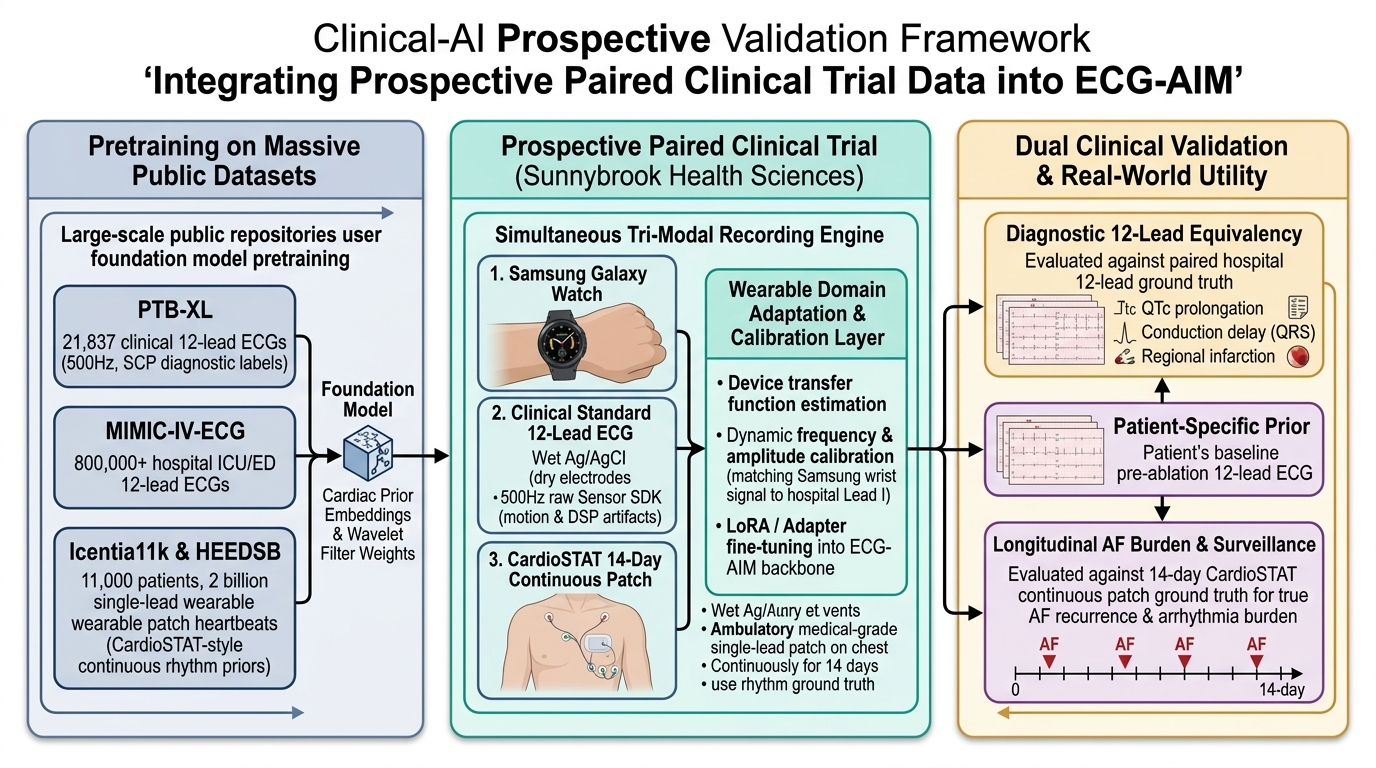
\includegraphics[width=\textwidth,height=0.76\textheight,keepaspectratio]{paired_trial_model_integration.png}
  \end{column}
  \begin{column}{0.46\textwidth}
    \vspace{-0.6em}
    \scriptsize
    \begin{itemize}
      \setlength{\itemsep}{0.2em}
      \item Pretraining on public cohorts (PTB-XL, MIMIC-IV, Icentia11k) to establish baseline representations.
      \item Data acquisition across three streams:
        \begin{itemize}
          \tiny
          \item Smartwatch: daily ambulatory ECG and in-clinic paired Lead I.
          \item CardioSTAT patch: 14-day continuous monitoring at 3 and 6 months.
          \item Hospital 12-lead machine: routine clinical tracings at each visit.
        \end{itemize}
      \item Hardware transfer function estimation and adapter calibration on paired recordings.
      \item Evaluation on distinct endpoints:
        \begin{itemize}
          \tiny
          \item Primary: AF recurrence and burden relative to CardioSTAT patch.
          \item Secondary: 12-lead waveform reconstruction and repolarization tracking.
        \end{itemize}
    \end{itemize}
  \end{column}
\end{columns}
\note{
  Figure 3 shows how the clinical trial and AI engineering integrate.
  Stage 1 represents foundation models pretrained on public datasets.
  Stage 2 represents data acquisition: smartwatch, 14-day continuous CardioSTAT patch, and hospital 12-lead machine.
  Stage 3 uses the paired in-clinic data to calibrate the hardware transfer function and adapt the model.
  Stage 4 shows the separation of endpoints: primary clinical AF surveillance vs. secondary translational 12-lead reconstruction.
}
\end{frame}

% ------------------------------------------------------------------------------
% Slide 18: Sample Size, Statistical Power & Clustered Modeling
% ------------------------------------------------------------------------------
\begin{frame}{Sample Size, Statistical Power \& Clustered Modeling}{Sample size justification and statistical analysis plan}
\begin{columns}[T]
  \begin{column}{0.48\textwidth}
    \begin{block}{\textbf{Primary Clinical Power (Protocol v1.1)}}
      \scriptsize
      \begin{itemize}
        \setlength{\itemsep}{0.2em}
        \item Primary outcome: time to confirmed AF recurrence.
        \item Hypothesis: smartwatch surveillance is non-inferior to 14-day patch monitoring.
        \item Event rate assumptions: 20\% recurrence with patch, 25\% with smartwatch.
        \item Target power: 80\% power, $\alpha = 0.05$, 10\% non-inferiority margin ($N=96$ patients).
        \item Vanguard phase: initial 20 consecutive patients to evaluate workflow feasibility.
      \end{itemize}
    \end{block}
  \end{column}
  \begin{column}{0.48\textwidth}
    \begin{block}{\textbf{Secondary AI Precision \& Analysis Plan}}
      \scriptsize
      \begin{itemize}
        \setlength{\itemsep}{0.2em}
        \item Sample yield: 96 patients across 4 clinic visits provides $>2,500$ paired complexes.
        \item Precision target: bounds QTc estimation error within 95\% CI margin of $\pm 3.5$\,ms.
        \item Within-patient beat clustering violates independent observation assumptions.
        \item Linear mixed-effects models (unstructured covariance) and generalized estimating equations (GEE).
      \end{itemize}
    \end{block}
  \end{column}
\end{columns}
\vspace{0.3em}
\centering
\scriptsize
{\color{NavyPrimary}Primary sample size is powered on clinical event rates; secondary analysis accounts for repeated measures.}
\note{
  This slide outlines sample size and statistical considerations.
  The primary clinical trial sample size of 96 patients is calculated directly from expected AF recurrence rates—20% on patch vs 25% on smartwatch with an 80% power target.
  For the secondary AI aim, 96 patients across multiple clinic visits provides over 2,500 paired cardiac complexes.
  Per Riley's 2024 BMJ guidelines, this is sufficient to bound QTc measurement error within a 3.5 ms margin of error.
  We specify linear mixed-effects models and generalized estimating equations to adjust for intra-patient beat clustering.
}
\end{frame}

% ------------------------------------------------------------------------------
% Slide 19: Action Items & Alignment for Today's Meeting
% ------------------------------------------------------------------------------
\begin{frame}{Discussion Points \& Open Questions}{Items to align on before protocol amendment}
\begin{columns}[T]
  \begin{column}{0.50\textwidth}
    \begin{block}{\textbf{Protocol Decisions}}
      \scriptsize
      \begin{enumerate}
        \setlength{\itemsep}{0.25em}
        \item Protocol structure: Confirm two-track design separating Aim 1 (AF recurrence) from Aim 2 (translational AI).
        \item In-clinic paired recording: Approve 5-minute simultaneous smartwatch + 12-lead acquisition at four scheduled visits.
        \item Secondary biomarker: Finalize priority endpoint for paired analysis (QTc tracking is our current recommendation).
        \item Vanguard phase: Authorize 20-patient feasibility cohort to evaluate workflow and data pipeline.
      \end{enumerate}
    \end{block}
  \end{column}
  \begin{column}{0.46\textwidth}
    \begin{block}{\textbf{Practical Feasibility Questions}}
      \scriptsize
      \begin{itemize}
        \setlength{\itemsep}{0.25em}
        \item \textit{Device/phone pairing}: Samsung Galaxy Watch requires a Samsung smartphone. Do participants need to own one, or does the study provide devices?
        \item \textit{CardioSTAT as fine-tuning data}: Can patch recordings at 3 and 6 months be used to condition patient-specific model adaptation?
        \item \textit{Paired data timing}: Which clinical visit is most logistically consistent for 12-lead + smartwatch co-recording?
        \item \textit{Consent scope}: Does the existing ethics approval cover secondary AI analysis on in-clinic recordings?
      \end{itemize}
    \end{block}
  \end{column}
\end{columns}
\vspace{0.3em}
\centering
\scriptsize
{\color{NavyPrimary}Next step: Finalize protocol amendment text and ethics consent addendum; initiate vanguard enrollment.}
\note{
  To close our meeting, here are the key decisions and open questions.
  On the protocol side:
  First, confirm the two-track design: Aim 1 is Chris's AF recurrence trial; Aim 2 is the secondary AI reconstruction aim.
  Second, approve the 5-minute in-clinic paired recording procedure.
  Third, decide which secondary clinical biomarker to prioritize—QTc tracking is our recommendation.
  Fourth, authorize the 20-patient vanguard.
  On the practical side, there are four questions we need to address:
  One: Samsung Galaxy Watch pairs only with Samsung smartphones. Most patients will not own a Samsung phone. We need to decide whether to restrict enrollment to Samsung phone users, provide phones, or switch to a cross-platform wearable (e.g., Fitbit, which pairs via Android or iOS). This has direct implications for consent, enrollment eligibility, and per-participant cost.
  Two: CardioSTAT recordings collected at 3 and 6 months provide a second source of patient-specific single-lead data per individual. This could be used to fine-tune a low-rank adapter on each patient's individual electrophysiology before deploying the reconstruction model—but this would need to be pre-specified in the analysis plan.
  Three: Which clinic visit is most operationally reliable for the paired recording? Baseline may involve more staff and time pressure; 3-month follow-up is likely lower acuity.
  Four: Does the current REB approval cover secondary AI analysis on in-clinic recordings, or do we need a consent addendum? This should be clarified before data collection begins.
}
\end{frame}

\end{document}
